\documentclass[12pt,a4paper]{article}
\usepackage{setspace}
\usepackage{amsmath}			
\usepackage[utf8]{inputenc}		
\usepackage[T1]{fontenc}			
\usepackage[english]{babel}			
\usepackage{graphicx}			
\graphicspath{{images}}
\usepackage{subfigure}				
\usepackage{lscape}					
\usepackage{pst-plot, pstricks}		
\usepackage{fancybox,amssymb,color}	
\usepackage{setspace}				
\usepackage{booktabs}
\usepackage{longtable}	
\usepackage{adjustbox}	
\usepackage{multirow}		
\usepackage{float}	
\usepackage{lipsum}
\onehalfspacing
\pagestyle{plain}
\setlength{\parindent}{1em}
\setlength{\parskip}{1ex}
\usepackage[%  
colorlinks=false,
pdfborder={0 0 0},
linkcolor=black
]{hyperref}

\usepackage{geometry}   		 % definition of the page layout
\geometry{
	a4paper,					 % format
	left=25mm,					 % left margin
	right=25mm,					 % right margin
	top=25mm,					 % distance upwards
	bottom=25mm,				 % distance downwards
	includehead,				 % distance from upwards till the page header
}
					

% Setting for the enumerate environment. Replaces the sub numbering of alphabet with numbers 
\renewcommand{\theenumi}{\arabic{enumi}}
\renewcommand{\labelenumi}{\theenumi}
\renewcommand{\theenumii}{\arabic{enumii}}
\renewcommand{\labelenumii}{\theenumi.\theenumii}
\renewcommand{\theenumiii}{\arabic{enumiii}}
\renewcommand{\labelenumiii}{\theenumi.\theenumii.\theenumiii}
\renewcommand{\theenumiv}{\arabic{enumiv}}
\renewcommand{\labelenumiv}{\theenumi.\theenumii.\theenumiii.\theenumiv}


\begin{document}
\begin{titlepage}
\begin{center}
	\noindent{\LARGE{A characterization of Colombian industries under Schumpeter's patterns of innovation }} \\
	\vspace{0.75em}
	\textbf{\large{Bachelor Thesis}} \\
\end{center}
\begin{center}
	\textit{by} \\
	\large{Juan José Taborda-Núñez}\footnote{8th Semester Economics student at Universidad del Norte (Colombia). \href{mailto:jtabordaj@uninorte.edu.co}{jtabordaj@uninorte.edu.co}}
\end{center}


\vspace*{\fill}
\begin{abstract}
The literature has continuously examined the relationship between market structure and innovation. Particularly, Joseph Schumpeter’s Mark I and Mark II innovation patterns inquired on what type of firm drives innovation based on competitive structures. Schumpeterian patterns of innovation have been widely used in the literature to classify productive sectors. However, said exercise is missing in periphery economies like Colombia, thus, this article will inquire in this matter by classifying Colombian industries across the secondary sector. 

Through a k-means clusterization algorithm, industries are grouped based on three measures, similar to those employed in the literature: Stability of innovation, Technological Opportunities and Market Concentration. Clusterization yielded two groups of industries (CG1 and CG2). Both descriptive and inferential statistics assessed the features of each and provided evidence to argue in favour of CG1 as Mark II industries and CG2 as Mark I industries. Several policy implications are discussed afterwards, among these, the need for a differentiated approach for specific segments within the secondary sector. Sectoral relationships, strategic relevance to the country or historical features are key points to consider when elaborating incentive architectures that address the sectoral heterogeneity found in the research, in order to foster adequate environments for innovative activities to develop. 
\end{abstract}

\vspace*{\fill}
	\vfill{
		\normalsize
		\flushleft
		\begin{tabular}{@{\qquad}llll}
			Supervisor 1: & Prof. Dr. Jana Schmutzler & Course: & Taller de Investigación \\
			Supervisor 2: & Prof. Dr. Werner Bönte & Course Professor: & Prof. Dr. Juan Perilla \\
			Submitted: & \today & Aspiring title: & BSc Economics
		\end{tabular}
	}
\vspace*{\fill}
\end{titlepage}

\newpage

\vspace*{\fill}

\begin{center}
	\textit{This page is intentionally left blank}
\end{center}

\vspace*{\fill}

\pagebreak
	
	
% ============================================================================================================================
% Lists
% ===========================================================================================================================
\pagenumbering{roman}
\tableofcontents \newpage
\listoffigures
\listoftables \newpage
\pagenumbering{arabic}
\setcounter{page}{1}


% ============================================================================================================================
% Main text
% ===========================================================================================================================

\section{Introduction and problem statement}
	
Who drives innovation within an industry? Is it a small firm or an established one? Is it an incumbent business or a novel startup? According to mainstream economics, several factors influence. For example, market structure, entry barriers, specialization and patent legislation. The presence and interaction of these factors may concentrate or disperse efforts, disincentivize novel ideas in favour of established paradigms, place industries at the source of a supply chain, motivate cooperation, and foster the appropriation of gains from innovation.    

For the case of a developing country, this article will answer this question using Joseph Schumpeter’s (1911;1942) Mark I and Mark II innovation patterns. Both archetypes assess a different market structure. While Mark I argues that novelty does not enter markets at the hand of incumbent firms but by entrant firms or new startups, Mark II appoints not the bold new enterprise or the brave startup but the large corporation as the driver of innovation.  

As with every theory, its importance relies on its results when tested empirically. Fontana et al. (2012) pointed out an untapped potential for Mark I and Mark II patterns in this field. Moreover, existing characterizations for both Marks have “\textit{been standing the test of time quite well}". There has been progress on characterizing industries with this pattern (Breschi et al., 2000; Castellaci and Zheng; 2010; Malerba and Orsenigo, 1996), which in turns gives a better insight of innovative activities in the countries where it takes place and serves as platform for policymakers to set up better guidelines for innovation-related policies.  

But Fontana et al. (2012) fail to notice the concentration of this type of study across the globe. Even though there are contributions to fill this gap worldwide, assessments in some countries are missing, with emphasis on countries outside the global north and core economies such as Colombia.   

A gap in characterization eventually leads to a need for information. Hence, this document will employ information contained in DANE (2020) “\textit{Encuesta de Desarrollo e innovación tecnológica}” (EDIT) survey and DANE (2019) “\textit{Encuesta Anual Manufacturera}” (EAM) survey for manufacturers to characterize industries as Mark I or Mark II, according to their International Standard Industrial Classification code (ISIC, or CIIU in Spanish), focusing on Section C: Manufacturing.  

This goal sets an intriguing task. First, there is novelty as earlier attempts to characterize all Colombian industries through Schumpeter patterns of innovation seem to be missing. Second, the characterization of industries yields useful information for future works and policymaking for one of the most important sectors in the country. Bear in mind that Colombian manufacturing has a 10\% share on its GDP (Gross Domestic Product), but accounting for aggregated value chains, it composes more than one-third of the economy (Arbelaez et al., 2021). With all things considered, the objectives and question of this research are: 



\begin{center}
	Research Question: \\  \textbf{Based on Schumpeterian Mark I and Mark II archetypes, who drives innovation within Colombian manufacturing industries?}
\end{center}


\begin{enumerate}
	\item \large Using Joseph Schumpeter’s Mark I and II innovation archetypes, employ quantitative methods to characterize Colombian industries within the manufacturing sectors as Mark I or Mark II industries, in order to inquire on the drivers of innovation constrained to market structure and industrial dynamics.
\begin{enumerate}
	\item \normalsize Combine information from the EDIT and EAM surveys to set up a database about firm features in manufacturing industries.
	\item Based on EDIT and EAM information, construct a quantitative analysis at the firm level that yields a result at the industry level, which in turn gives groundwork to create industry-level comparisons.
	\item Employing a cluster algorithm, group industry-level data by common patterns and characterize them using Schumpeter's Mark I and II.
	\item By analyzing intra-sectoral trends and geographical distribution, argue about potential policy implications and recommendations for adequate incentive architectures or industrial policies that foster a suitable environment within industries for innovative activities to occur.
\end{enumerate}
\end{enumerate}

\pagebreak

\section{Theoretical Framework}

\textbf{The concept of innovation and its taxonomies }

The base of innovation-related studies is to set up the concept of innovation and innovative activities. It is important to note that these concepts are contested in the literature, however, for the purposes of this research, we will employ the OECD (2018) concept of innovation as a "\textit{New or improved product or process (or a combination thereof) that differs significantly from the unit's previous products or processes and that has been made available to potential users (product) or brought into use by the unit (process)}" (p. 20).  

Although the OSLO handbook points out that innovation is inherently subjective —and therefore an ongoing debate in the literature exists— its practical application is objective if we consider the shared motives of novelty, utility and the ability to demonstrate significant differences. In that sense, the OSLO manual defines innovative activities as "\textit{all developmental, financial and commercial activities undertaken by a firm that is intended to result in an innovation for the firm}" (p. 20). Despite being a firm-centric perspective, OECD's concept can also apply to markets and industries. Moreover, OECD specifies whether innovation is for improvements on business practices, productive processes, goods, services, and marketing.  

Innovation may have two taxonomies based on its novelty and impact. Schumpeter (1942) focused on the nature of radical innovations as departing from known opportunities looking to forge something new at the expense of destroying something old. Schumpeter's perspective of innovation would create the concept of creative destruction. On the other hand, Kirzner (1973) argued that human alertness to new opportunities yields more rents when channeled into incremental innovations, those who do not compromise the \textit{status quo} and work under the realm of known opportunities. 

The OSLO manual reinforces the concept of radical innovations as those that transform the status quo. Moreover, it adds disruptive innovations such as those that take root in simple applications of niche markets and then diffuse throughout them. Disruptive innovations do not immediately compromise the status quo but eventually displace established firms (OECD, 2018, p. 78). For this research, we will employ the concepts of radical innovations as those that alter the status quo and have the potential to displace established firms and incremental innovations as those that stem from improvements to existing ideas that do not alter the current paradigm of the market  

\pagebreak

\noindent \textbf{Schumpeterian patterns of innovation }

It was not the OECD that introduced innovative patterns. It was Schumpeter (1911; 1942) who explored these differences and pioneered the proposal of differentiated archetypes for innovation. In his 1911 book "\textit{The Theory of Economic Development}", he employs a metaphor that sums up his early thoughts on new combinations and who carries them: "\textit{new combinations are, as a rule, embodied, as it were, in new firms which generally do not arise out of the old ones but start producing beside them; (…) in general it is not the owner of stagecoaches who builds railways}" (p. 66). The premise of Schumpeter implies that novelty does not enter the market at hands of incumbent firms but by entrant firms. This idea would be coined as Schumpeter's Mark I, which places entrant firms as the drivers of innovation.

Schumpeter's ideas would change later in his 1942 book "\textit{Capitalism, socialism and democracy}", where he reflects on previous perfect competition remarks and contrasts it with continuous standard of life improvements during the era of unrestrained “\textit{big business}”. By going into the details of this phenomenon, Schumpeter finds out that the trail of recent productive improvements leads to the door of large corporations, and: "\textit{ (...) a shocking suspicion dawns upon us that big businesses may have had more to do with creating that standard of life than with keeping it down}" (p. 82). Such perspective departs from Mark I and will become Schumpeter's Mark II. In contrast to a Mark I market, Schumpeter appoints large, established firms as the driver of innovation. It is not the bold new enterprise or the brave startup that brings new goods or services but the tried and true stable, large corporation. Schumpeter would reinforce Mark II later in the book: "\textit{Perfect competition is not only impossible but inferior and has no title to being set up as a model of ideal efficiency}" (p. 106).   

\noindent \textbf{Market structure and innovation }

Mark I and II may seem exclusive. They are not exclusive \textit{per se}, but the subjacent market structures they are. According to Fontana et al. (2012), one may classify industries using Mark I and Mark II archetypes. Mark I industries are turbulent, with low entry barriers and fiercer competition. On the other hand, stable environments with large established firms and entry barriers characterize Mark II industries. In other terms, Schumpeter's Mark I and Mark II describe the two fundamental market structures and their relation to who drivers of innovation. Mark I approach perfect competition, while Mark II appeals to a monopolistic (or oligopolistic) structure. 

With an established framework using Schumpeter's contributions we can now add up its patterns with OECD's taxonomy. Two propositions may aid in this. First, Gilbert (2006) states that the incentive to innovate is the difference in profits that a firm can earn if it decides to do so. Second, said profits, according to Arrow (1962), are higher in perfect competition than in monopoly, because the existing monopoly power acts as disincentive for innovation. Perfect competition seems to have suitable incentives to introduce breakthroughs in the market. Baumol (2004) reinforces this idea by saying: “\textit{major breakthroughs have tended to come from small new enterprises}” (p. 10). In that sense, risky innovations that seek to disrupt the \textit{status quo}, which OECD labels as radical innovations, seem to relate perfect competition structures, which appeals to a Mark I pattern.  

Baumol (2004) observation continues: “\textit{(…) while the invaluable incremental contributions that multiply capacity and speed and increase reliability and user-friendliness have been the domain of the larger firms}” (p. 10). This allows us to construct the definition of the market structure related to incremental innovations. By considering Arrow’s replacement effect and Gilbert statement on innovation incentives, we have strong signals that incremental innovations suit concentrated markets. Surely, entry barriers and high resource endowments deter potential entrants, but when it comes to innovation, monopolies have less incentives to change the paradigm of their markets, as it threatens existing gains. Therefore, incremental enhancements, as Baumol exemplifies, that increase reliability or user friendliness, characterize concentrated markets. In this case, the innovation pattern appeals to Mark II.  

As an overlook of both Schumpeter’s and Arrow’s theories, Shapiro (2012) remarks that the unifying principle of both is that a contestable market and potential profits from sales spur innovation. Moreover, a firm that wants to maintain the \textit{status quo} (e.g., Monopolies) has a smaller incentive than new entrants (let it be, a small startup) to disrupt said status by introducing radical innovations. 

Features of each archetype will be useful in our quantitative analysis, as it tells us what to look for in the data. To sum things up, we can say the following for each archetype: 

- Mark I: Related to perfect competition structures on which start-ups, small and new firms are the drivers of innovation. Radical innovations tend to be the signature type of innovation on this archetype, as firms have enough incentives to capture the market through new goods or services. This produces a highly competitive, turbulent and unstable environment in which firms are looking for ways to capture the market through a disruption of the \textit{status quo}.  

- Mark II: Appeals to concentrated market structures (e.g., monopolies or oligopolies) on which large firms are the drivers of innovation. Incremental innovations are in the line with this market, as they do not compromise established paradigms, but rather enhance what already exists. The resulting structure is a concentrated, stable, and less competitive market in which new ideas and innovations are disincentivized as they threaten the dominant position of incumbent monopolies or oligopolies. 

\noindent \textbf{Quantification of Schumpeterian patterns of innovation}

After Schumpeter, multiple concepts to quantify its patterns have been employed. Most of these variables are constructed at the firm-level, but they can be aggregated to construct industry-level metrics. Thus, they are good measures for describing firm features and market structures. For example: 

\begin{enumerate}
	\item \textit{Stability of innovation}: Refers to the degree on which the \textit{status quo} within a market can be disrupted through innovation. Hence, unstable environments are those on which radical innovations are more common than incremental innovations. In contrast, stable environments are more likely to have a larger share of incremental innovations compared to radical innovations. Stability usually employs a dynamic approach, seeking to identify the behaviour of innovation within an industry over time. 
	
	\item \textit{Entry and exit rate of firms}: It is also a dynamic approach. It captures at which rate firms enter and exit a certain market on a time frame. This can shed light on a market’s degree of competition. A market in which dominance is determined by competition will have greater entry and exit rates, as fierce competition can drive weak firms out of the market constantly, but also attract new ones. On the other hand, a market in which a few dominant firms hold their position through entry barriers and other deterrence methods will evidence low entry and exit rates, as incumbent firms do not face fierce competition and their position is rather secured. 
	
	\item \textit{Market concentration}: Traditionally, it refers to either the share of output or sales that a firm has within an industry. Market concentration is a common market metric to measure whether an industry is concentrated in a few firms or dispersed across a wide range of players. High market concentration is often viewed as a sign of stability and low competition, as one or a few agents controls most of the resources in the market, thus having significant control over it. In contrast, low market concentration is associated with turbulence and instability, as several players control small shares of a market resources, with no clear leader.  
	
	\item \textit{Degree of appropriability}: Appropriability captures the usage of protection mechanisms to appropriate the gains from an invention. Protection mechanisms tend to raise barriers to knowledge, but also incentive agents to innovate, as they have a degree of certainty that their invention can yield benefits. 
	
	\item \textit{Technological Opportunities}: It represents what opportunities the market has by evaluating how many protection mechanisms have been registered across a specific time set or relative to two discrete time periods. A high degree of technological opportunities is usually represented by several protection mechanisms being registered, while a low degree of opportunities behaves in the opposite way.
	
	It is important to acknowledge a bidirectional causality on this matter. Since appropriability refers to ability to protect, and technological opportunities refers to usage of protection, high usage of protections implies high ability to protect and vice versa. Thus, a relation between both variables exists.
\end{enumerate}

Numerous referents have tested these measures in the contexts of Schumpeterian patterns of innovation. To give a couple of examples, Malerba and Orsenigo (1996) approach, and eventually, Breschi et al. (2000) work tested variables such as concentration, entry, firm size, hierarchy of innovators and turbulence of markets. Malerba and Orsenigo (1996) approach also explored a relation between appropriability and technological opportunities.

On the other hand, Maleki et al. (2018) used patenting growth rate as a measure for technological opportunities. Similarly, Fontana et al. (2021) inquires into technological opportunities, but also on accumulativeness and appropriability of knowledge. Finally, Castellaci and Zheng (2010), productivity analysis approach focuses on appropriability and technological opportunities, discriminating by mode and source.\footnote{We shall find appropriability modes by the names of "conventional" and "non-conventional" protection mechanisms later on in this article.}

Quantification of Schumpeterian patterns will prove to be a cornerstone of the methodology, as all of its measures come from the theoretical body discussed in this subsection.

\noindent \textbf{Innovation systems and spatial analysis}

An innovation system is a set of interactions that foster, create, transform and diffuse knowledge on a specific territory. Nelson (1993) was one of the first authors to introduce this concept at the national level (NIS), Malerba (2002; 2003; 2005) introduced them at an industry or sectoral level (SSI), and D’Allura et al. (2012) reviewed regional systems (RSI).

Innovation systems may expand our understanding of Schumpeterian patterns of innovation by including an spatial component. This concept echoes with urban and spatial economic analysis. As firms agglomerate and configure their activities around physical sources of inputs (labour or raw materials), capital (financial markets or fixed capital), infrastructure (ports or railways) and geographical conditions (presence of mountains, rivers or roads), they also agglomerate to exploit non-tangible interactions like economies of scale, institutional coverage and spillover effects. 

Schrempf et al. (2012) identify two main interactions, one with government offices, and the other with higher education. Besides these, they acknowledge that policy incentives, regional governance and informal institutions, like culture and folklore, influence how and where industries configure in the territories.

This implies that regions are not equal when seen through the lens of innovation. Territories in neighbouring regions, or even within the same region exchange and foster knowledge differently. A complex and simultaneous set of interactions between several agents transmits information to markets about how profitable or adverse a specific territory may be for innovative activities.

At a policy-making level, RSI supports the "no one‐size‐fits‐all" policy instruments. That implies that an innovation policy accounting for RSI must be context‐wise, adapting to regional circumstances, either by targeting market failures, facilitating interactions, or streamlining institutional governance. 

Sectoral systems of innovation (SSI) have a mechanism of interactions similar to those found on RSI. However, SSI interactions are much more narrow. According to Malerba (2003), they emphasize on everything around the invention, creation and diffusion of a specific product from that sector. In that sense, the demand of physical inputs, like labour or raw material, together with intangible interactions, like knowledge diffusion, positive externalities, organizational structures and research cooperation strive towards enhancing, producing and selling specific products. 

Therefore, agglomerations are suitable proxies for those territories favouring that activity in particular. For example, a RSI analysis may find a specific city or region as a cluster of several agents, but a SSI analysis will probably be more narrow and precise on identifying those territories where that specific activity is favoured. After that, policy making may inquire on the reasons behind it and build suitable incentive architectures or institutional relationships that favour that product specifically.

We shall borrow some elements of innovation system later on, when discussing potential policy implications of our findings, based on spatial analysis and sectoral regional distributions.

\section{Literature Review}

Market structure as a determinant of innovation has been a recurrent topic in literature. Authors like Loury (1979) modeled innovation on an equilibrium environment, its results advocate for a market with finite number of competitive firms for innovation incentives to reach their optimal levels, the author prefers this point even though the number of firms is below the perfect competition rule of entry until profits are zero. Loury (1979) also suggests that atomistic competition is the market structure that provides optimal levels of innovative activities. 

Mansfield (1963) acknowledged a relationship between firm size, concentrated markets and share of innovative activities, where the share of new inventions is disproportionally carried out by large firms. This is based on three propositions: costs of innovation are high and only large firms can afford it, innovation needs a large scale so success and failure can balance out, and firms need sufficient control of a market to properly reap the gains from their innovations. Its empirical findings support these propositions, but find them not universally true, as some industries report less concentrated market share of innovative activities, giving more space for middle and small firms to innovate. 

Raider (1998) finds that a combination of market structures and adversity drives innovation. The author’s results show that firms facing high pressure from market competition tend to innovate more, whereas markets without this phenomenon tend to innovate less. Raider (1998) does not use the traditional market concentration measure for innovation alone, but also takes a network market approach, showing that network constraints of buyers and sellers, together with extreme downstream and upstream competition within a market are determinants of innovation. 

A first prominent characterization exercise comes from Malerba and Orsenigo (1996), who identified Schumpeter’s Mark I and Mark II across 49 technological classes of six countries: the US, Japan, Germany, France, the UK, and Italy. The authors find Mark I as a widening pattern, where concentration of innovative activities is low, with small sized firms and low stability in the ranking of innovations. On the other hand, they find Mark II as a deepening pattern: high market concentration, larger firms, a stable ranking of innovators and deterrents to entry.

Further contributions by Breschi et al. (2000) suggest that better appropriability conditions work in the direction of Schumpeter’s Mark II pattern, while the opposite appeals to Schumpeter’s Mark I. Their contributions do align with earlier results by Malerba and Orsenigo (1996), reinforcing their findings. By means of a principal component analysis, they found that the ability to employ protection mechanisms to protect innovation has a positive relation with Schumpeter Mark II. Moreover, low market concentration reinforces widening patterns (Mark I), and high stability appeals to Mark II.   

Fontana et al. (2012) connects with Breschi et al. (2000) contributions. They employ similar measures in their econometric exercise, and their results maintain Mark I as the disperse and turbulent archetype, while Mark II as the stable and concentrated pattern. Landström \& Schön (2010) report a similar distinction of both patterns, but they add to the discussion similarities between them. For example, innovation is central to economic development and in both cases the capitalist assumes the risk.  

However, Schumpeter marks are not alone in the literature. Pavitt (1984) proposed an alternative to Schumpeter’s Mark I and Mark II archetypes. Pavitt's Taxonomy classifies industries based on the requirements of its users, the sources of its technologies, and the degree of appropriability. Pavitt finds four different patterns for industries: Supplier-dominated sectors; scale-intensive industries employing process and product innovation; specialized suppliers that market technology to other firms; finally, science-based, knowledge industries with a high degree of appropriability and tailored towards exploring innovative technological breakthroughs.  

One may ask which framework is better. However, both appeal to distinct aspects of the same subject. In the case of Pavitt’s taxonomy, Archibugi (2001) finds that each one closely ties with Kondratiev's long waves of capitalist development. On the other hand, Castellacci (2008) links Pavitt’s framework to the sectors that sustained the growth of advanced economies in the Fordist age. In contrast, Schumpeter's Mark I and II appeal to the dynamics of an industry life cycle. Mark I characterize the early stage of an industry, where turbulence in competition is common and there is no clear leader. On the other hand, Mark II refers to a more mature, late-stage phase of an industry that has large firms deeply rooted in the market (Malerba, 2005). 

In the literature, authors like Fontana et al. (2021), Breschi et al. (2000), Castellaci and Zheng (2010), Malerba and Orsenigo (1996), Corrocher et al. (2007), among others focused their efforts on Schumpeter's patterns. In contrast, Landström \& Schön (2010), Marsili and Verspagen (2002), and Leiponen and Drejer (2007) preferred an approach using Pavitt's taxonomy. 

The selection of either Schumpeter’s or Pavitt’s framework relies usually on the scope and objectives of the research. Researchers do share common ground in this matter, like using data from innovation-related databases or employing similar econometric approaches, but the purposes vary. For example, Breschi et al. (2000) borrowed elements from Malerba and Orsenigo (1996) but narrowed its study to three countries and omitted control variables for the effects of a country's national innovation system. Corrocher et al. (2007) aimed to create a distinction for ICT sectors (instead of manufacturing) based on Schumpeter’s work, proving a coexistence of both Marks in some cases. Castellaci and Zheng (2010) deployed an industry-level productivity growth characterization using Schumpeterian patterns, where the research does not focus only on innovation, but also on elements of productivity like total factor productivity, technological and efficiency change. 

The literature has found that sometimes Schumpeter’s pattern may offer a narrow view of an industry, which makes them employ Pavitt’s taxonomy. Such is the case of Van Dijk (2000), who showed how some groups among Dutch manufacture do not fit easily into either group of Schumpeter’s Marks, which would result on incomplete analysis. Thus, Pavitt taxonomy seems more suitable in this case. Leiponen and Drejer (2007) find a similar phenomenon on Danish industries, but they also face a problem on data availability. 

It is important to notice that, when researchers characterize multiple countries (e.g, Germany, the UK, France, the US, et cetera), they acknowledge specific country differences in their measures. For example, Malerba and Orsenigo (1996) were aware of country-specific effects related to national systems of innovation (NIS) and historical evolution of national firms and industries. Thus, they employ “\textit{dummy}” variables to capture the causal effect of these phenomenon in their study. Breschi et al. (2000) also employ “\textit{dummy}” variables to capture country-specific effects, however, as we stated previously, they diverge from Malerba and Orsenigo (1996) methods, as the variables capture the role of public procurement or consumer-producer interactions instead of innovation systems. 

Characterizing exercises yields information on how industries work around innovation and what environment they enclose. Policymaking can borrow elements from these studies. However, as we stated previously, tension builds in countries or regions where this exercise does not exist. With the emphasis on Colombia, Schumpeter's theory is known, as some articles appeal to its contributions (Umaña-Aponte et al., 2013; Marroquín, 2010; Arroyo-Mina \& Guerrero, 2018; Langebaek-Rueda \& Vásquez, 2007). Nonetheless, it is not used for characterization of industries but for impact evaluation, behavioral economics, and case analysis. There are attempts to build sector-specific entrepreneurship profiles (Cerón et al. 2010), and innovative profiles (Ovallos-Gazabón \& Amar-Sepúlveda, 2014), but they do not employ Schumpeterian patterns of innovation.  

Something else to consider is that Colombia is a peripheral economy. Based on the Dependence Theory (Ahiakpor, 1985) and empirical evidence (Arezki et al., 2013), we may argue in favour that the way in which markets structure in peripheral economies differs from developed and core economies. While in the former low added-value goods flow outwards and high-value goods flow inwards through imports, the latter does the opposite. Therefore, both industrial and innovative activities configure themselves in function of these flows. 

With that in mind, a problem may arise if we characterize peripheral economies under core economies frameworks. This is why Pavitt’s Taxonomy may be non-suitable to assess these types of countries, as it inquires on industrial features proper of advanced economies, like science-based sectors and specialized high-tech. Moreover, it takes as quantitative input specialized information that may be missing in developing economies. For example, technological sources, user requirements and appropriability regimes. 

Schumpeterian archetypes, on the other hand, may be more flexible for this analysis, due to its particular focus on two things. First, it answers what type of firm drives innovation through common market metrics like market concentration, firm size, or stability of innovation. Second, per Malerba (2005) observation, it may shed light on the dynamic of an industry, whether it is in an early stage, or it is entering a late phase of maturity.  

All things considered, this article will join the academic dialogue about innovation patterns in Colombia by characterizing industries in the manufacturing sector using Schumpeter's framework, a more flexible and suitable approach for a peripheral economy, which can supply an adequate insight into how firms behave toward innovation, based on the drivers of innovation, industrial life cycle and dynamics. In the following section, we will expand the methods of this research, including data sources, variable summary and clusterization method. Moreover, we will examine the limitations in terms of quantitative inputs that further reinforce the selection of Schumpeter’s patterns over Pavitt’s taxonomy. 


\section{Methodology}

This research employs a cross-section combination of DANE (2020) “\textit{Encuesta de Desarrollo e innovación tecnológica}” (EDIT) survey and DANE (2019) “\textit{Encuesta Anual Manufacturera}” (EAM) survey. EAM is a national census of firms that fulfill its classification criterion of at least ten employees and sales greater than 517 million pesos. If a firm fulfills the sales requirement but not the employee's requirement, it is also included in the census. Both surveys differentiate firms by a “\textit{Numero de Orden}” (NORDEMP) registration, which makes it easier to identify common patterns and merge them in one single database. 

Something else to consider is that the survey captures geographical information, as firms report the department where they are located. This information is organized using a "\textit{DIVIPOLA}" classification elaborated by DANE (2022) for geospatial analysis, where each department has an unique number. While this is not crucial for an initial cluster analysis, we can make use of this information after the cluster, in order to assign each firm within industries a geographical location for further policy recommendations.

On the other hand, the EDIT survey tackles the need for information about the type of innovative activities (radical or incremental) a firm undertakes, and their effects on performance such as cost reductions or productivity enhancements. There is data about sources of financing, information usage, human capital qualities, usage of patents, copyright, and other non-conventional protection methods. According to the DANE (2020) methodological overview, the EDIT survey preserves a theoretical framework that follows most of the methodological guidelines of the Organization for Economic Cooperation and Development (OECD), with emphasis on its innovation-tailored OSLO Manual. Annex 1 shows, at a four-digit ISIC level, the universe of study for the EDIT survey.  \footnote{Source: Own elaboration based on DANE's Methodology (2018, p. 7)}\footnote{As an exception, ISIC codes 202 and 210 select specific four-digit industries within them}. 

Given the fact that EDIT samples EAM sectors, instead of firms, not every industry in EAM is present in the EDIT. By using statistical software like R, such setback is solved through an inner join of both databases by their common ISIC code and NORDEMP registrations. Thus, the yielding database reduced the number of observations from almost 8000 to 6405.  

Based on some of the variables from Breschi et al. (2000), and Malerba \& Orsenigo (1996) studies, a Schumpeterian pattern of innovation can be measured using three dimensions: Stability, Technological Opportunities and Concentration. We will focus on those variables across both EAM and EDIT surveys that are similar in construction to the measures utilized in previous studies for these dimensions. As each observation is linked to a NORDEMP registration, it makes it easier to operate them. These variables are summarized in the following table:  

\begin{longtable}{lcll}
	\caption{Relevant variables for the study}
	\cr \hline \multicolumn{1}{c}{\textbf{Dimension}}                                                  & \textbf{Concept}                                                                                                          & \multicolumn{1}{c}{\textbf{Variable}} & \multicolumn{1}{c}{\textbf{Description}}                                                                                                                                                                                                         \\ \hline
	\multirow{2}{*}{Stability}                                                              & \begin{tabular}[c]{@{}c@{}}Amount of \\ radical \\ innovations\end{tabular}                                               & I1R4C2N                               & \begin{tabular}[c]{@{}l@{}}Goods and services that are \\ new or different from those \\ existing in the market, and \\ were introduced in the \\ 2017-2018 period.\end{tabular}                                                                 \\ \cline{2-4} 
	& \begin{tabular}[c]{@{}c@{}}Amount of\\  incremental \\ innovations\end{tabular}                                           & I1R4C2M                               & \begin{tabular}[c]{@{}l@{}}Goods and services that are \\ improvements to existing \\ goods or services in the market, \\ and were introduced in the \\ 2017-2018 period\end{tabular}                                                            \\ \hline
	\multirow{4}{*}{Concentration}                                                          & Total sales                                                                                                               & I3R2C1                                & \begin{tabular}[c]{@{}l@{}}Income or operational sales, \\ both local and foreign, \\ perceived by the firm between \\ 2017 and 2018. \\ In thousands of Colombian Pesos.\end{tabular}                                                           \\ \cline{2-4} 
	& \begin{tabular}[c]{@{}c@{}}Total spending on \\ innovative \\ activities\end{tabular}                                     & II1R10C2                              & \begin{tabular}[c]{@{}l@{}}Total investment by the firm \\ on innovative activities \\ for the 2017-2018 period.\end{tabular}                                                                                                                    \\ \cline{2-4} 
	& Total employees                                                                                                           & PERTOTAL                              & \begin{tabular}[c]{@{}l@{}}Permanent amount of employees \\ within a firm. Includes owners, \\ temporal employees and \\ permanent roster.\end{tabular}                                                                                          \\ \cline{2-4} 
	& Total Output                                                                                                              & PRODBIND                              & \begin{tabular}[c]{@{}l@{}}Firm output accounting for\\ the value of goods and services \\ at the end of the production process, \\ excluding intermediate goods.\\ In thousands of Colombian Pesos.\end{tabular}                                \\ \hline
	\multirow{3}{*}{\begin{tabular}[c]{@{}l@{}}Technological \\ Opportunities\end{tabular}} & \begin{tabular}[c]{@{}c@{}}Possession of \\ conventional \\ protection \\ mechanisms \\ valid until \\ 2018\end{tabular}  & VI1R8C2                               & \begin{tabular}[c]{@{}l@{}}Prior to the 2017-2018 period, \\ and valid until the end of said year, \\ how many conventional protection\\ mechanisms were in possession \\ of the firm.\\ Ex: Patents, IP, Copyright, \\ Trademarks.\end{tabular} \\ \cline{2-4} 
	& \begin{tabular}[c]{@{}c@{}}Obtention of \\ conventional \\ protection \\ mechanisms \\  between \\ 2017-2018\end{tabular} & VI2R8C2                               & \begin{tabular}[c]{@{}l@{}}Between 2017 and 2018, \\ how many conventional \\ protection mechanisms \\ did the firm acquire.\end{tabular}                                                                                                        \\ \cline{2-4} 
	& \begin{tabular}[c]{@{}c@{}}Usage of \\ non-conventional \\ protection \\ mechanisms\end{tabular}                          & VI3R5C2                               & \begin{tabular}[c]{@{}l@{}}Between 2017 and 2018,\\ how many non-conventional\\ protection mechanisms \\ did the firm acquire.\\ Ex: Non-Disclosure Agreement,\\ industrial secrets,\\ high complexity on design\end{tabular}                    \\ \hline


\end{longtable}
\begin{center}
	Source: Own elaboration based on DANE's (2019; 2020)  \\
\end{center}
\vspace{11pt}

 By operating these variables in R, three dimensions at the industry level are built: Concentration (\textit{CON}), Technological Opportunities (\textit{TO}) and Stability (\textit{STA}). A detailed explanation of each dimension, together with its proposed way to measure it, is listed below:  

\begin{enumerate}
	\item \textit{CON}: Based on the works of Malerba and Orsenigo (1996). It is a measure of concentration of innovative activities and firm size through the Herfindahl-Hirschman Index.  
	
	\textit{CON} will employ traditional variables in market concentration analysis such as total sales and total output. An additional variable to represent spending on innovative activities is also employed. Finally, a variable that measures the number of employees working in each firm also appears in the measure. Since concentration in these types of exercises not only refers to total sales or output, this dimension is built to expand the proposed dimension to give insight into how large firms are in terms of labour demanded for their productive activities, as well as how much financial resources they invest in innovative activities. 
	
	Variations between these each index are smoothened using a geometrical mean such that the industry-level measure adopts the form: 
		\begin{equation}
			\centering
			CON = (HH_{ms}*HH_{msa}*HH_{lsd}*HH_{ss})^{1/4}
		\end{equation}
	Where $HH$ is a Herfindahl-Hirschman index, and the subindex represents each measure of interest. In that sense, $ms$ means Market Share, $msa$ means Innovative Activities, $lds$ stands for Labour Demand Share, and $ss$ for Supply Share. Per our established conceptual review, we expect that low values of the CON measure will relate to Mark I industries, while large coefficients would appeal to Mark II industries. 
	
	\item \textit{TO}: Built using the Maleki et al. (2018) approach, where Technological Opportunities are measured by the growth rate of patents. However, growth rate requires a comparable measure for 2017. Since EDIT surveys are non-comparable, another measure is required. A similar approach is found by calculating the proportion of new protection mechanism relative to registered mechanisms. In this case, we can employ the following formula at the industry level:
	\begin{equation}
		\centering
		TO = \dfrac{PM_{1718} + NCPM_{1718}}{PM}
	\end{equation}
	Where $PM_{1718}$ captures the industry aggregate of all protection mechanisms obtained between 2017 and 2018, $NCPM_{1718}$ follows the same mechanism, but with emphasis on non-conventional protection mechanisms (e.g., Non-Disclosure Agreements, Industrial Secrets and Complex Design). Finally, $PM$ contains all protection mechanisms valid until the end of the year of interest (2018). 
	
	Technological opportunities have close ties with appropriability. A high degree of protection mechanisms signals high appropriability, whereas low tells the opposite. Considering Breschi et al (2000) distinction, Mark I industries have low appropriability for their inventions, while Mark II tend to appropriate knowledge better by employing more protection mechanisms. Based on that, we may speculate in favour of an inclination towards Mark II on industries with high TO values. 
	
	\item \textit{STA}: Since stability has close ties with firms entering and exiting the market of innovation, it demands a dynamic analysis. Bear in mind that DANE’s EDIT methodology states that EDIT 2018 is non-comparable with its predecessors. Thus, we need to employ a different approach.  
	
	In this case, we will make use of how many radical and incremental innovations a firm introduced to construct a quantitative measure at the industry level, by aggregating the observations of each firm. Based on the theory exposed previously, these two variables prove relevant to our study, as the composition of radical and incremental innovations can be used to shed light on how stable or unstable an industry is on its innovative activities. 
	
	\textit{STA} relies on Baumol (2004, p. 10) observation that “\textit{major breakthroughs have tended to come from small new enterprises, while the invaluable incremental contributions (…) have been the domain of the larger firms}.”. Baumol proposition, coupled with the relationship between firm size and Schumpeterian patterns established in the literature review, provides a stability approach that could be classified under either Mark I or II. Hence, to quantify that stability approach, the following mathematical form is proposed: 
	\begin{equation}
		\centering
		STA = Sr - Si
	\end{equation}
Where $Sr$ is the share of radical innovations over the total amount of innovations in the industry, and $Si$ the share of incremental innovations. Based on Baumol’s proposition and reviewed theory, we shall expect a high share of radical innovations to have a relation with turbulent Mark I industries, while incremental innovations to the Mark II archetype. 
\end{enumerate}

It is true that the literature has employed further measures to characterize industries such as firm entry and exit rates, patent registration as a proxy of technological appropriability, and changes in the ranking of top innovative firms as a measure of stability, among others. However, problems on data availability arise when attempting to measure these elements in Colombian manufacture, as data is incomplete, incompatible, or unavailable.  

Bear in mind that the fundamental basis to differentiate firms in this study is the unique NORDEMP registration, which allows us to bind information to a specific firm. NORDEMP usage is proper of DANE’s surveys and databases. This means that comparability with data obtained from other sources is difficult, as there is no reference point to determine which information belongs to which firm. 

Considering the nature of these three dimensions, some additional filters were implemented, as some industries, for example, reported an aggregate of zero on innovation activities spending. Therefore, the concentration measure would result in zero, even though the other components do report values greater than zero. This began to be a problem in industries with less than 20 observations. Hence, 20 becomes the minimum number of observations to classify in my study. A comprehensive table reporting three and four-digit ISIC industries included in my study, together with their results in each dimension, can be found on Annex 2 

The information is then clustered using a k-means method for 2 groups, employing a Lloyd algorithm and 10 repetitions. Following MacKay (2003) explanation, k-means calculates a mean for each group and assigns a data point (in this case, industry) to said group by the following mechanism: 

\begin{enumerate}
	\item \textit{Assignation phase}: Each observation gets assigned to the group with the closest mean (by Euclidean distance). Each generated group is composed by a centroid that serves as reference point for the following steps.  
	\item \textit{Update phase}: Group parameters adjust to match the means of the data points. 
	\item \textit{Repetition phase}: Assignation and Update phases repeat until they do not change anymore, that is, data points do not change their position in the groups. 
\end{enumerate}

Additionally, all information is standardized prior to the cluster calculation, using R native standardization method. This is made to prevent problems that may arise due to non-normalized euclidean distance, such as those noted by Martinez et. al. (1999):
\begin{enumerate}
	\item Distance sensibility: Euclid distance must be standardized to avoid overestimation by extreme values. If we consider our dataset of $i$ points, each point $x_{i}$ with a coordinate $\mu_{i}$, such as $x_{i} = \mu_{i}$, then its standardization, by definition, goes as follow:
	\begin{equation}
		\mu_{i} := \sigma \frac{x_{i}}{\sigma_{i}}
	\end{equation}
	Where $\sigma$ is an hypothetical measurement of standardization. If we consider that equation (4) normalized a data point by its standard deviation, then the standard deviation of the normalized dataset will be 1. This stems from the variance property:
	\begin{equation}
	\begin{split}
		Var(\alpha X) = Var(X)\alpha^2 \\
		Var(\frac{1}{\sigma} X) = \frac{Var(X)}{\sigma^2} \\
	    Var(\frac{X}{\sigma}) = \frac{\sigma^2}{\sigma^2} \\
	    = 1
	\end{split}
	\end{equation}
	With this in mind, the formulae of an Euclid distance $d$ between two vectors of points $q$ and $p$:
	\begin{equation}
		d = \sqrt{\sum_{i = 1}^{n}(q_{i}-p_{i})^2}
	\end{equation}
	Will adopt the form
	\begin{equation}
		d = \sqrt{\sum_{i = 1}^{n}(\sigma \frac{x_{iq}}{\sigma_{iq}} - \sigma \frac{x_{ip}}{\sigma_{ip} })^2}
	\end{equation}

	The resulting distance will be a $d$ value of $\sigma$ standard units. Thus, an initial standardization of the data yields a normalized Euclid distance. In other words, if we compute Euclidean distances on hypothetical $u'$ normalized coordinate vectors of our data, the resulting distances will be measured in units of standard deviations. This solves the distance sensibility problem.
	
	\item Redundancy by correlation: If variables are similar in construction, correlation may provide redundancy, and thus, overestimation of the distances. However, a previous calculation of Pearson correlation coefficients between $TO$ and $STA$, $TO$ and $CON$, and $CON$ with $STA$, yielded very low $\rho = 0.12$, $\rho = 0.08$ and $\rho = -0.17$ values respectively. In that sense, redundancy is minimal and the problem is not present.
\end{enumerate}

\section{The Cluster}
\subsection{Results}
\begin{figure}[H]	
	\caption{Characterization of Colombian Manufacture using a two groups k-means clustering method}
	\centering
	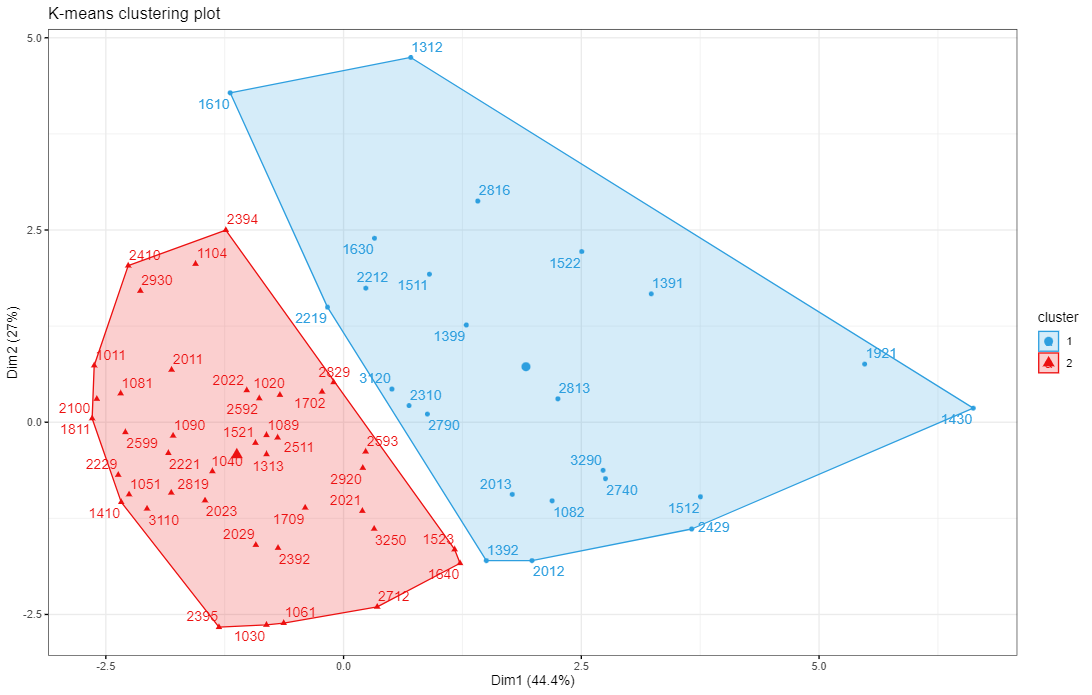
\includegraphics[scale = 0.45]{cluster.png}
	Source: Own elaboration based on DANE (2019;2020) databases.
\end{figure}

The previous figure shows the resulting cluster from the k-means algorithm. Before evaluating both groups, bear in mind that the X and Y axis are in function of “Dim1” and “Dim2” variables, instead of our initial measures. This change obeys to the fact that the k-cluster method in R employs a principal component analysis (PCA) dimensional reduction algorithm. PCA operates our three dimensions (\textit{STA, TO, CON}) and creates “shadow” variables "Dim1" and "Dim2". These variables capture a certain amount of the variation contained in the original dataset. In this case, Dim1 and Dim2 find components of 44.4\% and 27\% respectively. 

Cluster results show two groups. Cluster Group 2 (CG2), colored red, has 5192 observations and is denser than Cluster Group 1 (CG1), colored blue, which has 794 observations. On the other hand, red group industries are closer between them than those in the blue group. Initial descriptive statistics for both groups are shown in the following table. 

\begin{table}[h!] 
	\caption{Initial descriptive statistics of the two groups k-means clustering}
	\centering
	\begin{tabular}{@{}lllllll@{}} 
		\toprule 
		\multicolumn{1}{c}{} & \multicolumn{3}{c}{\textit{Cluster Group 2}}                   & \multicolumn{3}{c}{\textit{Cluster   Group 1}} \\ \midrule 
		
		& \textit{TO} & \textit{CON} & \multicolumn{1}{l|}{\textit{STA}} & \textit{TO}   & \textit{CON}   & \textit{STA}  \\ \cmidrule(l){2-7}  
		
		\textit{Max}         & 3.500       & 1023.11      & \multicolumn{1}{l|}{0.586}        & 6.000         & 2702.96        & 1.000         \\ 
		
		\textit{Min}         & 0      & 160.28       & \multicolumn{1}{l|}{-1.000}       & 0.047        & 1068.11        & -1.000        \\ 
		
		\textit{Mean}        & 0.522      & 572.22       & \multicolumn{1}{l|}{-0.294}       & 0.983        & 1507.72        & -0.345        \\ 
		
		\textit{Std Dev}     & 0.651       & 262.98       & \multicolumn{1}{l|}{0.414}        & 1.496         & 416.08         & 0.550         \\ \bottomrule 
	\end{tabular} \\ 
 	Source: Own elaboration 
\end{table} 

Differences arise on their descriptive statistics, which may aid in our characterization purpose. In the case of CG2, Technological Opportunities oscillate between a growth rate of 350\% and no growth at all, with a representative value of 0.52 and a standard deviation of 0.65. Concentration values in CG2 tend to be smaller, oscillating between 1023 and 160 on the Herfindahl-Hirschman index and reporting a representative value of 1507. Standard deviation across concentration stands at 262 index points. Finally, Stability reports values between 0.586 and –1 with a standard deviation of 0.414 and a mean of –0.294 

In the case of CG1, we find a large value of Technological Opportunities, with industries reporting a growth rate of 600\% relative to existing protection mechanisms. The mean of this group stands near 1 with a standard deviation of 1.496, telling us about an overall feature in this group to grow their protection mechanism registries more than their CG2 counterparts. Concentration index in CG2 also reports a significant deviation from CG1 results. While the former oscillates between 2702 and 1068, with a representative value of 1507, the latter passes maximum 1000 index points. Finally, Stability reports on average slightly higher values towards incremental innovations when compared to CG1.  

\subsection{Inferential analysis}

In this section, results are put in context with Schumpeterian patterns of innovation by employing further data visualization and inferences. To begin with, results report lower Stability in CG2 when compared to CG1. Even though the mean difference in both groups is not large, data distribution as per Figure 2 shows that the density plot for CG1 has a prominent number of observations between 0 and -1, which in turn means, by the nature of the measure employed, that CG1 has many industries with a predominance of incremental innovations in their aggregates. This remark is reinforced by a highly positive skew of the distribution. 

In the case of CG2, it distributes mostly below 0, but its differentiating factor is its lower density when compared to CG1 across said interval. Even accounting for non-extreme values —that is, excluding the lower and upper ten per cent of each distribution—, results remain consistent. Skewness and kurtosis measures further support this idea. 

The main insight to draw from this analysis is that CG1 industries tend to be dominated by larger shares of incremental innovations in their aggregate, while industries in CG2 do not show this tendency, instead, they have smaller differences between radical and incremental shares rather than disproportions towards one of the two types. Box plots support this conclusion, considering that CG1 left box is wider than its CG2 equivalent.

\begin{figure}[H]	
	\caption{Density and box plots of both Groups in the Stability dimension.}
	\centering
	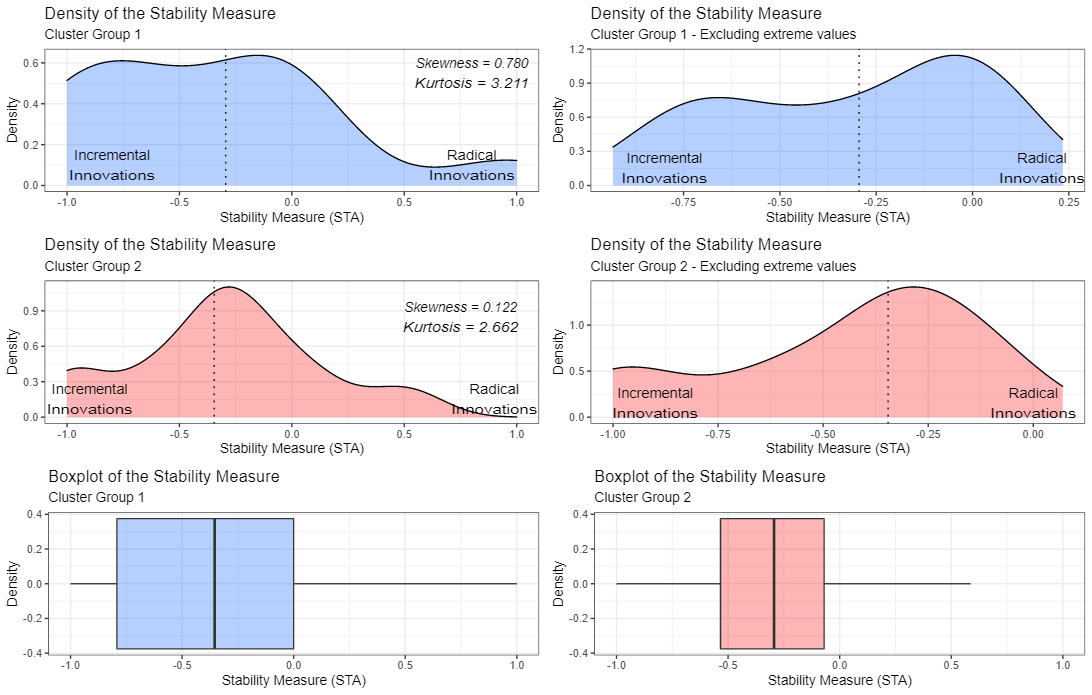
\includegraphics[scale = 0.45]{sta.png}
		Source: Own elaboration
\end{figure}

Within the Concentration measure, density plots in the next figure show a clear difference between both groups.  While CG2 distribution finds its peak near 500 and reaches 1000 concentration points at most, CG1 reports values above 1000, with a long-tailed right side until 2700. By excluding extreme values, this evidence persists. 

Boxplot of both datasets provides a different visualization of this phenomenon, but confirms that CG1 market concentration is, on average, much larger than industries on CG2. All this statistical insight points out to one conclusion: CG1 industries are highly concentrated, thus, dominated by larger firms. 

\begin{figure}[H]	
	\caption{Density and box plots of both Groups in the Concentration dimension.}
	\centering
	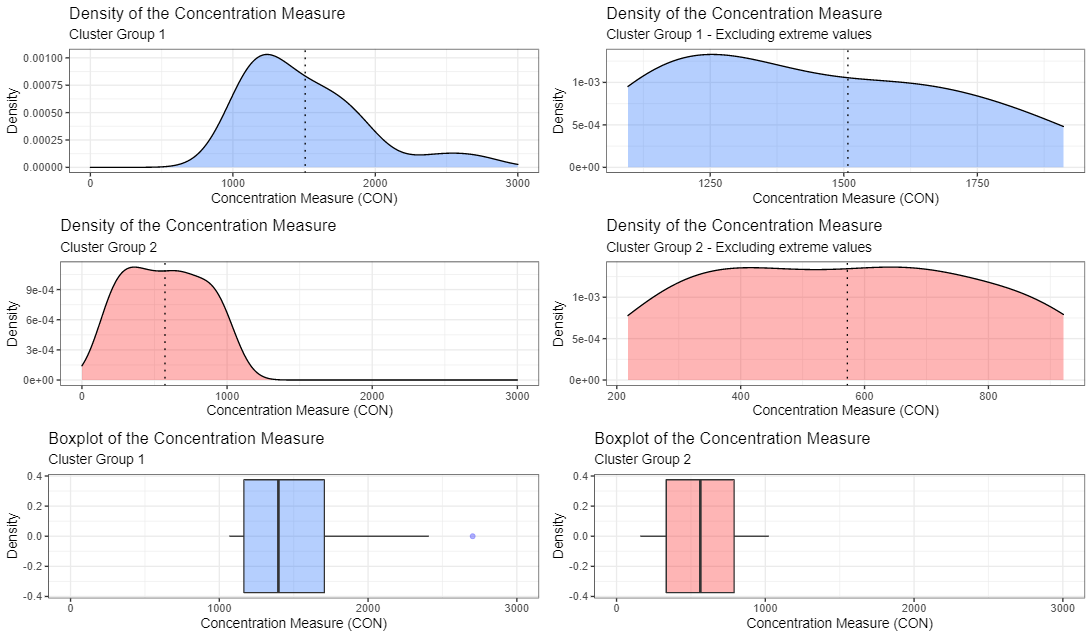
\includegraphics[scale = 0.45]{pcon.png}
		Source: Own elaboration
\end{figure}

Finally, the behaviour of technological opportunities shows that both groups distribute mostly near zero. However, as shown in the next figure, skewness in CG2 is larger than CG1, which may lead us to infer that their registry of new protection mechanisms relative to the existing ones is low, which in turn may indicate low appropriability. Kurtosis in CG2 is also higher, which indicates that the TO measure industries classified on CG2 is highly concentrated around its mean. 

In the case of CG1, both moments are lower. Thus, CG1 industries do register a higher proportion of protection mechanisms relative to the existing ones compared to CG2, which may indicate an overall higher level of appropriability in this group. Box plots reinforce this idea, as CG1 right box is wider. Expanding this inference exercise by excluding extreme values, we find a similar result. CG2 distributes mostly between 0 and 1, while CG1 spans wider, from 0 to 2.

\begin{figure}[H]	
	\caption{Density and box plots of both Groups in the Technological Opportunities dimension.}
	\centering
	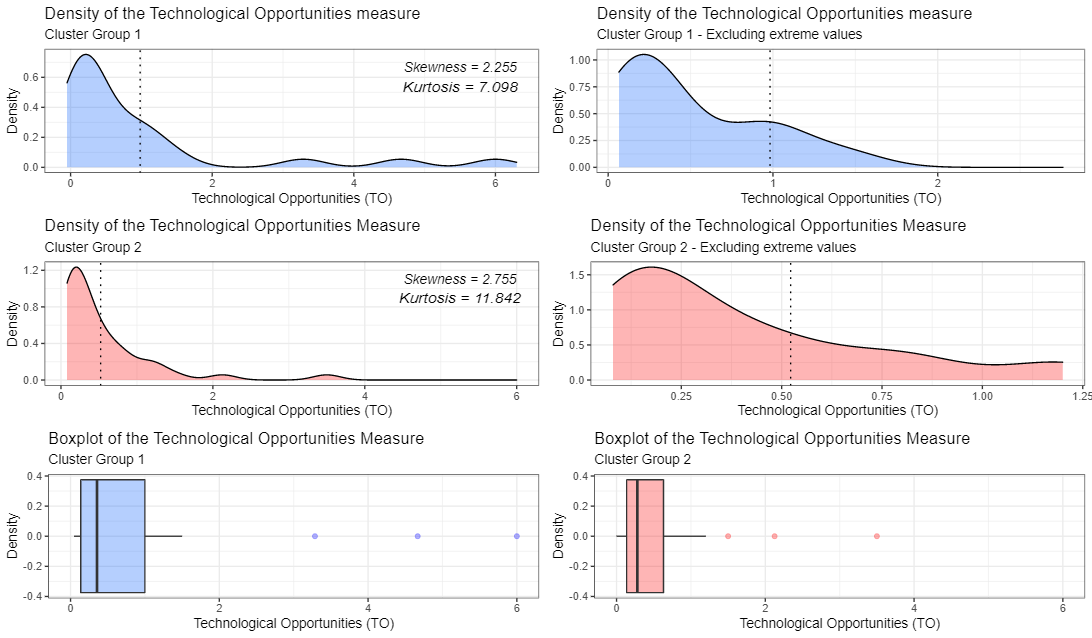
\includegraphics[scale = 0.45]{to.png}
		Source: Own elaboration
\end{figure}

By evaluating these three dimensions, let us go over again our most important discoveries. First, we found a trend in CG1 towards high shares of incremental innovations, while CG2 tends to be more balanced between shares. Second, CG1 market concentration is clearly larger in average than CG2, which in turn gives us reasons to argue in favour of large firms as the dominant agents of these industries. Finally, we found that CG1 industries register more protection mechanisms relative to the existing ones compared to CG2, which appeals to higher levels of appropriability as there are formal methods to secure benefits from innovation (e.g., Patents, IPs, Copyrights, et cetera). 

Per this inferential analysis, and based on reviewed theory, we can characterize CG1 industries under the Mark II pattern, while features of CG2 industries gravitate towards the Mark I Archetype. 

This analysis of results shows consistency with the literature reviewed in past sections. Theory on the quantification of Schumpeterian patterns, together with previous works from Malerba and Orsenigo (1996), Breschi et al. (2000), Fontana et al. (2012) can be validated.

Said studies agree on two things, first, Mark I as a widening, dispersed and turbulent environment, with less appropriability and low opportunities; Mark II is a deepening, concentrated and stable environment, where technological opportunities and appropriability are higher. Said features across both archetypes exposed in the literature are similar to those found within each cluster group, and the subsequent inferential analysis. We found a group that is, simultaneously, highly concentrated, with several registrations of protection mechanisms, high share of incremental innovations, and therefore, less turbulence. The other group (CG2),  is more disperse, with less protection mechanisms, and turbulence in the form of radical innovations.


With emphasis on each dimension, the literature employed in the methodology shows coherence with the results. Malerba and Orsenigo (1996) concentration approach is consistent in this work, and the expansion to include novel measures has not distorted it, as less disperse firms present features proper of Mark II industries, and vice versa for Mark I. Maleki et al. (2018) form for technological opportunities shows a similar behaviour. Finally, the proposition of a novel measure for innovation Stability, based on Baumol (2004) proposition yielded intriguing results. 


\section{Policy implications}

\subsection{Intra-sectoral trends}

By classifying industries in function of which firm drives innovation within them, we possess insights that may aid in the formulation of industrial policies. As we commented earlier on this research, due to its position as a periphery economy, commodities and first-generation manufacturing (textiles, clothing, footwear) are strategic sectors in Colombia, while advanced manufactures and technological appliances (computers, chipsets, telecommunications) are not. 

In this study, there is presence of industries dedicated to early manufactures and commodities, which prove strategic for the Colombian economy. For example, production of meat and fish products (101), general food products (102, 103, 104, 105, 108, 110), coffee (106), petroleum (192), metals and non-metallic minerals (239, 242, 251, 259, 241, 243), furnitures (311, 312), wood, paper and cardboard products (161, 163, 164, 170), and textiles (131, 139, 141, 143). \footnote{The numbers between parentheses represent either three or four-digit ISIC codes related to each sector or subsector. This information can be double-checked by referring to Annex 1 and 3} 

Results show that 9 subsectors within the food products industry behave as Mark I, meaning that small firms drive innovation. Only one exception in this segment arises, cacao and chocolates (1082) find itself in a Mark II environment, which could be related to Colombia's Nutresa group (formerly known as \textit{Nacional de Chocolates}) influence in the domestic market. Moreover, this trend implies that flagship industries in Colombia like Coffee elaboration, which sustained its early economic growth in the 20th Century (Luzardo-Luna, 2019), has dispersed efforts, low market concentration and less technological opportunities reflected in less appropriability. Innovation policies targeted to these sectors may find better results by focusing on the features and interactions that may occur within this type of environment. 

In the case of early manufactures like textiles, most subsectors find themselves with large concerns as the driver of innovation. Among these, weaving of textiles (1312), made-up articles for home and related (1392), knitting and crocheting (1391, 1430), and other textiles (1399). However, the most popular sector in this segment, the elaboration of wearing apparel (1410) using several types of materials (wool, leather, fabric, lace, et cetera) behaves as a Mark I industry. Similarly, finishing textiles (1313) through dyeing, dressing, drying or bleaching, behaves as Mark I. It is true that Mark II spans across several sectors, however, the two most important in this segment are not powered by large businesses when it comes to innovation.  

This is not the only case, other segments also report mixed results. For example, in furnitures, the elaboration of furnitures (3110) in general behaves as a Mark I industry, while the elaboration of mattresses (3120) behaves as a Mark II industry. In the case of wood, cardboard and paper products, sawmilling of wood (1610) and elaboration of wood components for building (1630) have large corporations at the spearhead of innovative activities. However, elaboration of wood (1640), cardboard or paper containers (1702), and other manufactures of the same concern, like household and office products (1709) operate under Mark I environments. 

A policy approach in this case should start by identifying the archetype of those sectors that sustain most of the productive activity in the country and build an incentive architecture around it. While  is true that most of the sectors in textiles behave as Mark II, the two most important in first-generation manufacturing behave as Mark I. A differentiated approach towards those that sustain the most is strongly advised, as the dynamics of these are different than the rest of their segment. 

Finally, other important commodities like petroleum, metals, rocks and related items present mixed results. Petroleum has only one subsector in the study, which is the manufacture of several fuel types used in modern industrial activities (1921), making it a crucial subsector within its industry. This study has found it to operate within a Mark II environment, coherent with sectoral evidence, where Colombian state-owned Ecopetrol captures a considerable part of the fuel market. In this case, the policy implication tends to gravitate towards incentives that favour the market leader. This is reinforced by the importance of the sector for modern activities. Favourable policies, together with suitable incentive architectures that lead to product or process improvements in this subsector have domino-effects in other sectors. As its final product is an input in other activities, an improvement here is an improvement in the cost structure of several firms. 

On the other hand, the segment of metals and non-metallic minerals has a trend of Mark I industries. Manufacture of clay (2392), cement (2394), concrete (2395), basic iron and steel (2410), structural metals (2511), hand tools (2592), metal coating (2593), among others (2599) have a Mark I environment. However, production and refining of non-ferrous metals like nickel, copper, lead, chrome, manganese, zinc, aluminium, among others (2429) operates as a Mark II subsector. 

In this case, subsectors that treat conventional metals or minerals (iron, steel, clay, cement, et cetera) tend to have dispersed efforts and less concentrated markets, but more specialized metals tend to be concentrated around the efforts of a small group of businesses. Policies in this case should bear in mind this distinction in order to favour development. Moreover, in contrast with petroleum, another thing to consider in policy-building is that output across these subsectors is widely used either as input in other activities or as a final good for consumption.    

\subsection{Sectoral regional distribution}

As we said earlier, we will borrow theoretical elements about innovation systems to expand our understanding of the clusterization exercise. This will be done by incorporating a detailed spatial analysis of the industries studied within this document. To begin with, the following figure shows the spatial localization of those industries within the segment of food products.

\begin{figure}
	\caption{Spatial distribution of colombian industries in the segment of food products}
	\centering
	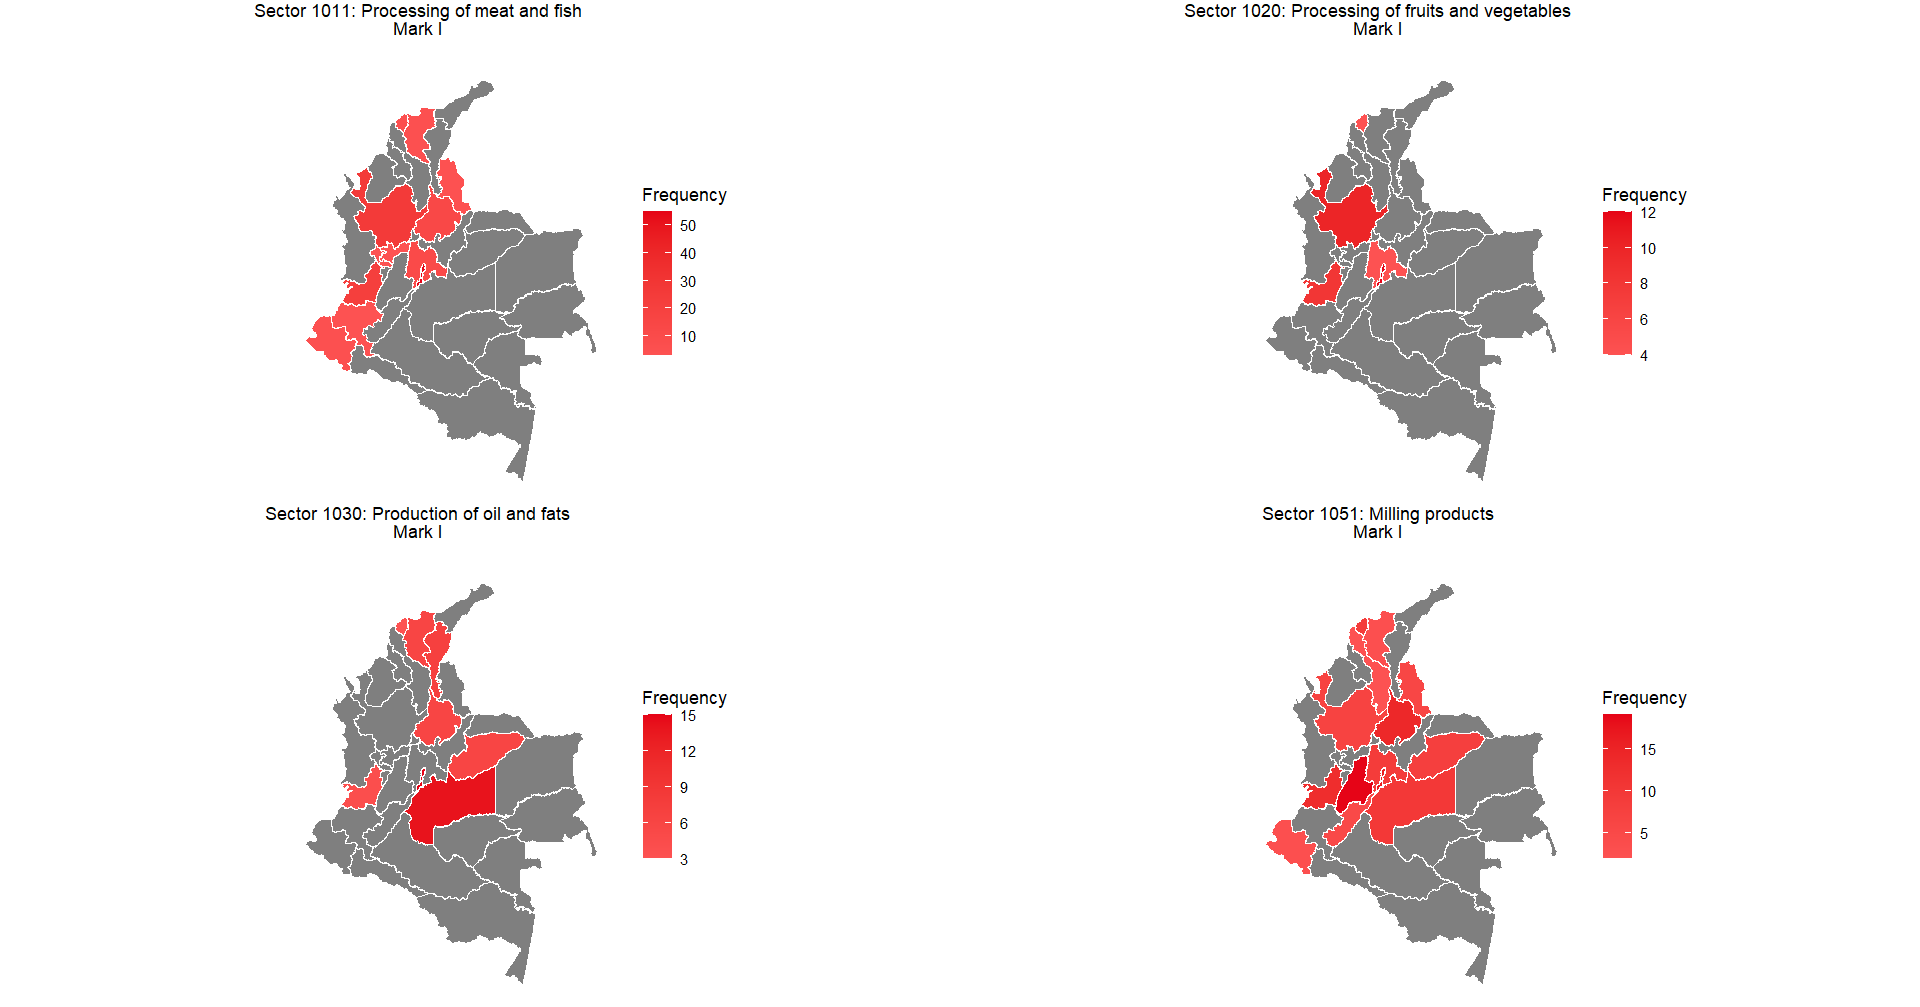
\includegraphics[scale=0.4]{fp1} \\
	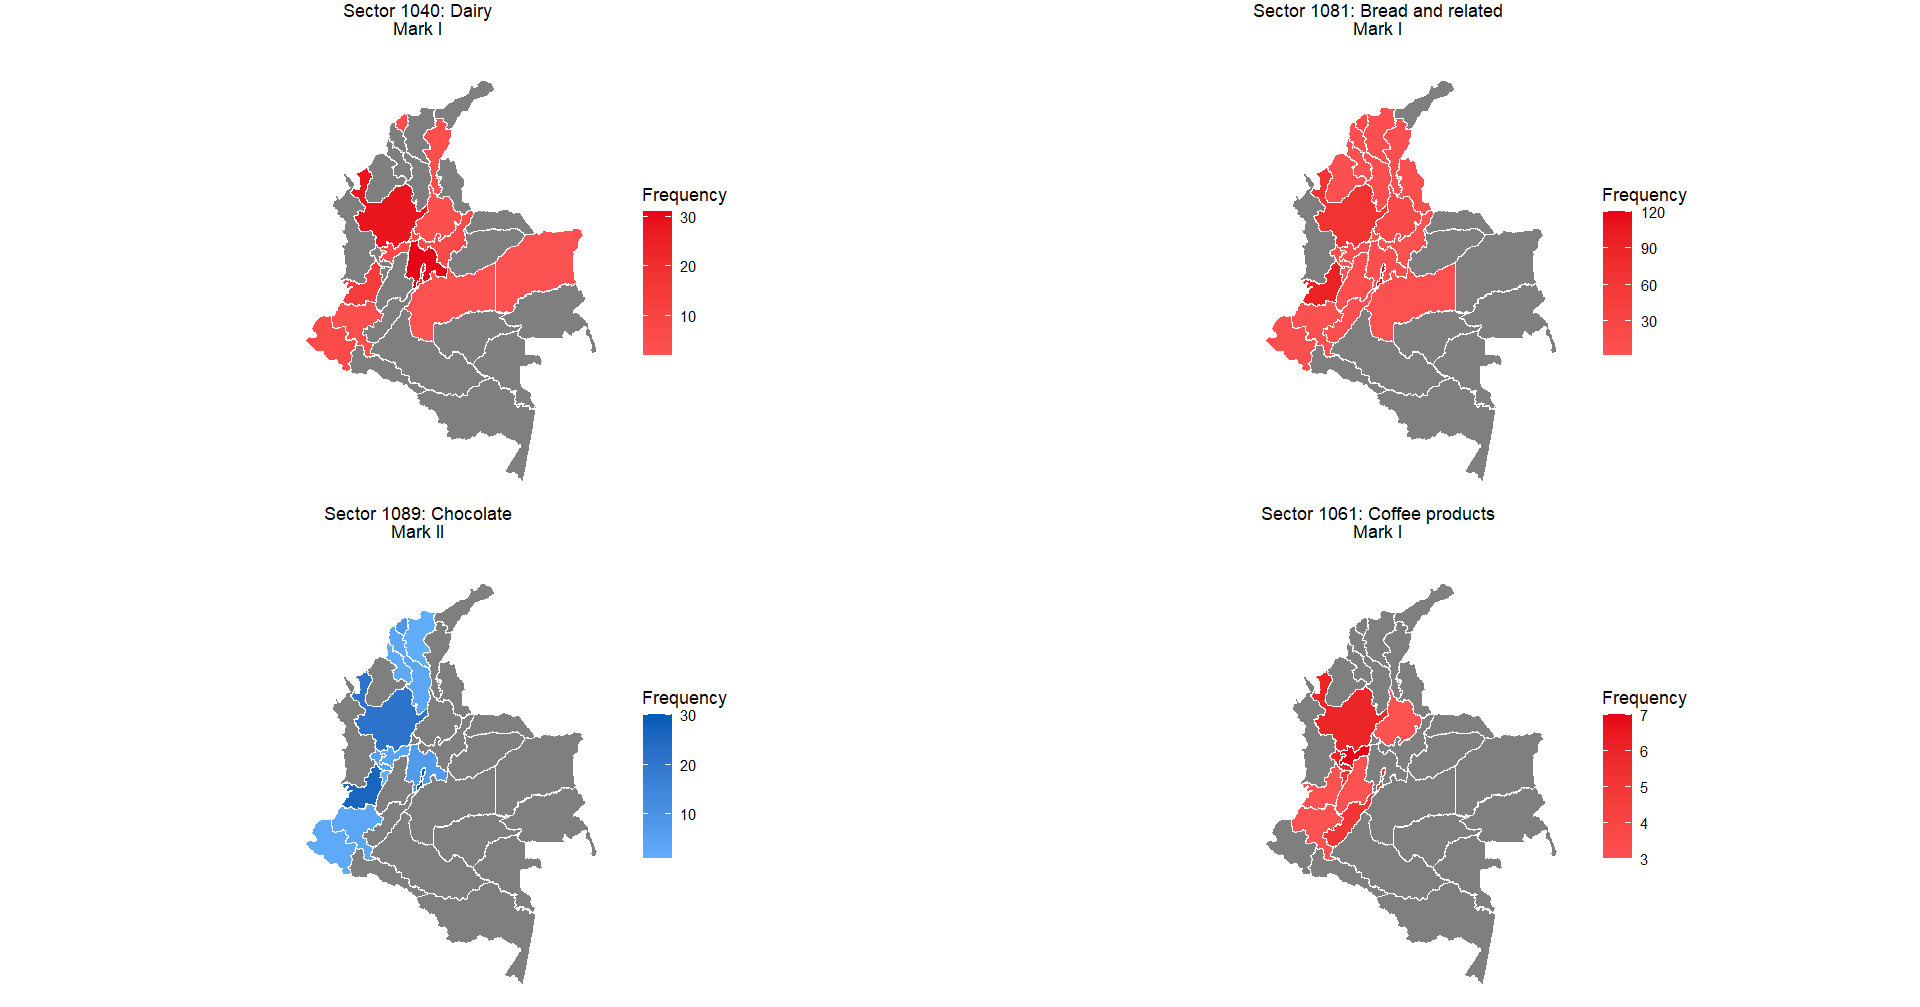
\includegraphics[scale=0.4]{fp2}
	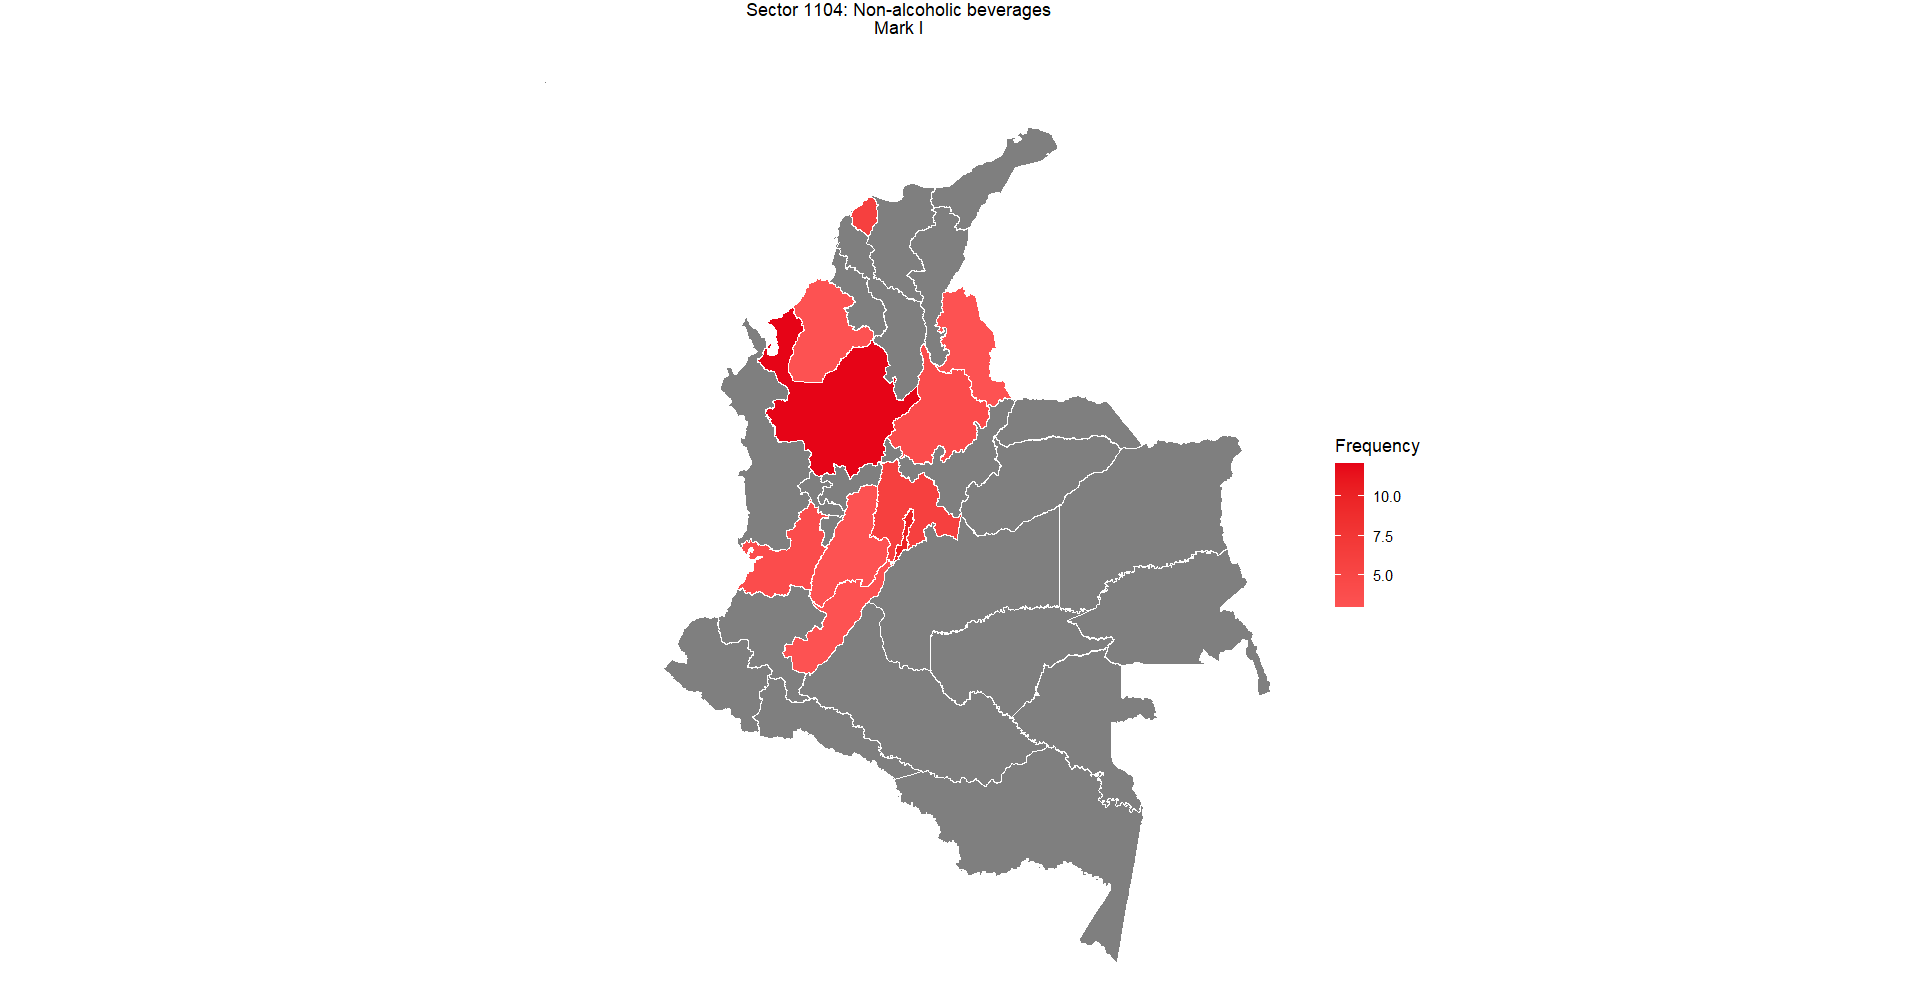
\includegraphics[scale=0.25]{sodas} \\
	Source: Own elaboration
\end{figure}

At a regional level, both the Andean and Caribbean region have the most number of agglomerations. Within both, Atlantico and Magdalena are the most repeated in the Caribbean, but the frequency of firms in this region does not compare to the Andean, where Bogota\footnote{Per Colombia's political-administrative partition, Bogota is a first-order territory, with its own administrative autonomy. Despite acting as the capital of Cundinamarca, its population size and administrative faculties requires distinction}, Antioquia, Cundinamarca and Cauca Valley (\textit{Valle del Cauca}) have the majority of firms. Frequency differences within the Andean region also arise, Antioquia reports a persisting trend of holding denser clusters of firms across sectors.

In this case of a predominantly Mark I segment, spatial distribution tends to span across several departments, but following a very fractionalized, this can be seen clearly on sectors like oil and fats (1030), fruits and vegetables (1020), dairy (1040) and milling products (1051). Production of bread and similar goods seems to be evenly distributed with Antioquia and Cauca Valley as leaders, nevertheless, this trend does not repeat anywhere else. The only Mark II industry (chocolates, 1089) spans across the Caribbean and Andean region without major breaks in the distribution, but with two dense centres in Cauca Valley and Antioquia.

Now, if we extend to a context-specific sectoral analysis, then we can draw further conclusions. For example, dairy (1040), together with meat and fish products (1011), agglomerate near valleys for livestock, or coasts for fish, but also near major urban centres, looking for easy access to transport hubs and other inputs. On the other hand, processing of fruits and vegetables locate near major cities (Cali in Cauca Valley, Barranquilla in Atlantico, Medellin in Antioquia and Bogota in Cundinamarca), and Coffee products (1061) show expected results, as the map points to agglomeration around the well-known Coffee Axis (\textit{Eje cafetero}). 

Moreover, institutional factors and transport routes seem to highly affect localization decisions. Industries not only find enough labour and capital inputs in major urban centres, they also benefit of nearby access to transport hubs (e.g \textit{El Dorado} airport in Bogota, Magdalena river and caribbean ports like Barranquilla or Cartagena), close distance to government authorities, and thus, an assured enforcement of the law. This seems to be a crucial factor on the firm decision to locate geographically.

In the case of textile products and wearing apparel, the following figure shows their spatial distribution. Results show much more narrow clusters, and this may provide evidence to reinforce the institutional factors that we discussed previously. Across all sectors in Mark II, and one in Mark I, dense agglomerations appear near major cities in central Colombia. Only the elaboration of wearing apparel (1410) is somewhat disperse, but even its dispersion falls within the Andean region centre, where institutional presence and law enforcement is higher than in peripheral regions. Centralism seems to be a strong political economy trend in Colombia, or at least in the elaboration of textiles

\begin{figure}
	\caption{Spatial distribution of colombian industries in the segment of textiles}
	\centering
	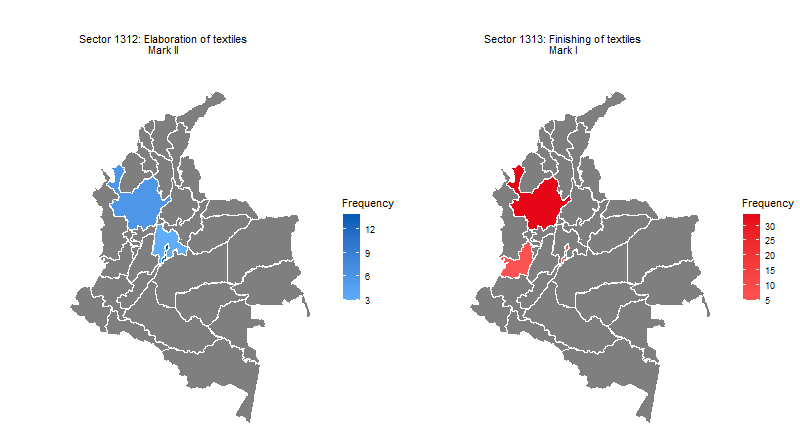
\includegraphics[scale=0.6]{et1} \\
	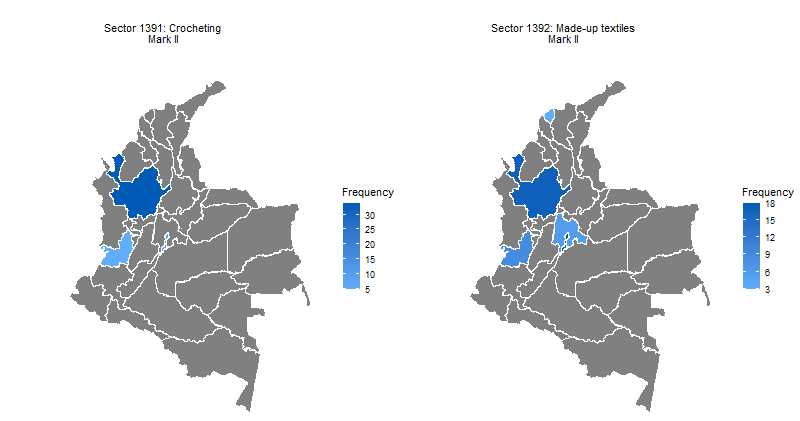
\includegraphics[scale=0.6]{et2} 
	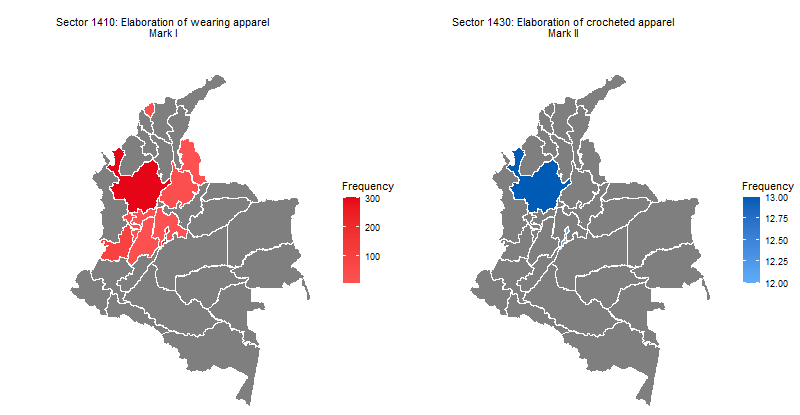
\includegraphics[scale=0.6]{et3} \\
	Source: Own elaboration
\end{figure}

On the other hand, Antioquia reinforces its position as the department with most agglomerations. Cauca Valley and Cundinamarca (including Bogota) follow. The Caribbean coast and some regions on the east dissapeared from the map in this segment. Antioquia's position echoes with its 19th and 20th century economic history. As noted by Ocampo (2015) and Luzardo-Luna (2019), hard-currency profits from coffee exports, human capital formation, informal ties between citizens, railway infrastructure, and other resource endowments consolidated Antioquia as an industrial powerhouse, with domestic concerns like Coltejer (\textit{Colombiana de tejidos}) and Fabricato (\textit{Hilados y tejidos del hato}). Results in this article show that this consolidation persists until today, even despite  fiercer foreign competition due to trade liberalization.

We now turn our attention to the segment of... WIP




% Notes: big firms dont spread geographically may indicate dependance on institutional enforcement. Policy to spread institutions > spread firms > spread productive activities
% But also big cities tend to have better infrastructure and thus better access to both domestic and foreign markets
% Textiles reinforce that ^
% First segment seem to have cauca and antioquia as leaders overall and in the Andean. Bogota follows in the Andean. Atlantico and magdalena seem to be of interest in the caribbean but are smaller in density
% Second segment consolidates antioquia as main cluster, Cauca Valley and Cundinamarca follow. Labour inputs, tap potential markets and access to resources may explain??

\section{Conclusions and final remarks}

Our conclusions revolve around four ideas. First, we have been able to characterize Colombian industries under Schumpeterian patterns of innovation. Even without the dynamic component of previous characterization exercises, statistical analysis and inference show clear differences, proper of Schumpeterian patterns. This adds weight to the main purpose of the study and introduces an aspect of Schumpeterian theory (innovation archetypes) to Colombian industries, and reinforces Fontana et al. (2012) proposition that Schumpeterian patterns stand the test of time quite well.

Second, we found what type of firm drives innovation on each industry. CG1, the less dense group, has been labeled as Mark II, thus, larger firms drive innovation within this group. On the other hand, CG2, the densest group, gravitates toward Mark I, placing startups and small firms as the drivers of innovation. This difference in amount shows us that Colombian manufacture is more of a Mark I than Mark II sector, as the largest group of industries is the Mark I group.  

Third, our measures are consistent to what was exposed in the theory and literature. For the Colombian case, concentration is the spearhead of innovation pattern analysis, as the most prominent differences came from its measure. It is true that the Stability and Technological Opportunities measures yielded relevant results, but its analysis required further statistical tools to produce a formidable conclusion. Among these, we had to employ statistical moments like kurtosis or skewness coefficients, together with kernel distributions excluding upper and lower 10 per cent values, to provide clear inferences and conclusions. 

Finally, policy implications discussed in the last section of the paper tend to identify specific segments of productive activities across Colombia’s economy. Sectors like groceries are predominantly characterized as Mark I, including Colombia’s flagship coffee sector. Textiles are predominantly Mark II, but that does not necessarily imply that the most important sectors follow this trend, because the elaboration and finishing of wearing apparel has a Mark I environment. Oil, one of the most important commodities in the modern world, is a Mark II industry, appealing to the prevalence of state-owned Ecopetrol as the most important firm in the domestic market. A similar phenomenon occurs in the chocolate market, with Nutresa's market dominance. Other commodities and early manufactures, like wood and metals report trends specific to their segments. 

\textbf{MAPPING CONCLUSIONS HERE}

The main takeaway from the policy implication section is that policy makers should bear in mind a differential scope. No one policy type will work across the entire secondary sector. It is important to consider specific sectoral relationships, usage of goods as inputs or final consumption, strategic relevance to the country, historical features and importance on the consumption basket of final users. Incentive architectures should be designed in function of addressing this sectoral heterogeneity to foster adequate market environments for innovative activities to develop. The means to achieve this purpose vary, but a comprehensive set of policy measures or incentive architectures should include tax incentives, patent and trademark protection, anti-trust regulations, competition laws, among others... 

To sum things up, this article deployed a characterization exercise across Colombia’s secondary sector using Schumpeter’s Mark I and II as framework, a k-means clustering as method, and three dimensions based on existing literature as the measures. Results provide an input for future works, either in the of advanced economic analysis (e.g, Econometric models) or for public policy elaboration. In the former, as industries are now classified under a Schumpeterian pattern of innovation, it may serve as the starting point for a probabilistic or regression exercise, in the latter, as we found who drives innovation within each industry, it may aid in future policies or reforms that tackle, for example, innovative activities or research incentives. I pointed out potential elements of a comprehensive set of policy measures to achieve this purpose, however, a comprehensive detail of each would exceed this article’s purpose. Thus, this gap may serve as another starting point for future inquiries on this matter. 


\pagebreak

\section*{References}
\emergencystretch 5em
\raggedright
{\setlength{\parindent}{-1.7em}
	\-\footnotesize.
	\normalsize

Ahiakpor, J. C. W. (1985). The Success and Failure of Dependency Theory: The Experience of Ghana. International Organization, 39(3), 535–552.

Arbeláez, M. A., Becerra, A., \& Benítez, M. (2021). Contribución fiscal y tributación efectiva de la industria manufacturera en Colombia. http://www.repository.fedesarrollo.org.co/handle/11445/4071

Archibugi, D. (2001). Pavitt’S Taxonomy Sixteen Years On: A Review Article. Economics of Innovation and New Technology, 10(5), 415–425. https://doi.org/10.1080/10438590100000016

Arezki, R., Hadri, K., Loungani, P., \& Rao, Y. (2013). Testing the Prebisch-Singer Hypothesis Since 1650: Evidence from panel techniques that allow for multiple breaks. In OxCarre Working Papers (No. 124; OxCarre Working Papers). Oxford Centre for the Analysis of Resource Rich Economies, University of Oxford. https://ideas.repec.org/p/oxf/oxcrwp/124.html

Arrow, K. (1962). Economic Welfare and the Allocation of Resources for Invention. In The Rate and Direction of Inventive Activity: Economic and Social Factors (pp. 609–626). Princeton University Press. https://www.nber.org/books-and-chapters/rate-and-direction-inventive-activity-economic-and-social-factors/economic-welfare-and-allocation-resources-invention

Arroyo-Mina, J. S., \& Guerrero, D. (2018). Schumpeterian Behavior in a CPR Game: Experimental Evidence from Colombian Fisheries Under TURF’s Management. Mediterranean Journal of Social Sciences, 9(4), Article 4.

Baumol, W. J. (2004). Entrepreneurial Enterprises, Large Established Firms and Other Components of the Free-Market Growth Machine. Small Business Economics, 23(1), 9–21. https://doi.org/10.1023/B:SBEJ.0000026057.47641.a6

Breschi, S., Malerba, F., \& Orsenigo, L. (2000). Technological Regimes and Schumpeterian Patterns of Innovation. The Economic Journal, 110(463), 388–410. https://doi.org/10.1111/1468-0297.00530

Castellacci, F. (2008). Technological paradigms, regimes and trajectories: Manufacturing and service industries in a new taxonomy of sectoral patterns of innovation. Research Policy, 37(6–7), 978–994. https://doi.org/10.1016/j.respol.2008.03.011

Castellacci, F., \& Zheng, J. (2010). Technological regimes, Schumpeterian patterns of innovation and firm-level productivity growth. Industrial and Corporate Change, 19(6), 1829–1865. https://doi.org/10.1093/icc/dtq051

Cerón, C. A., Alcazar, F. L., \& M, J. J. G. (2010). Caracterización emprendedora de los empresarios en los Valles de Tundama y Sugamuxi. Boyacá (Colombia). Pensamiento \& Gestión, 29, 163–189.

Corrocher, N., Malerba, F., \& Montobbio, F. (2007). Schumpeterian patterns of innovative activity in the ICT field. Research Policy, 36(3), 418–432. https://doi.org/10.1016/j.respol.2007.01.002

D’Allura, G., Galvagno, M., \& Mocciaro Li Destri, A. (2012). Regional Innovation Systems: A Literature Review (SSRN Scholarly Paper No. 2180119). https://papers.ssrn.com/abstract=2180119

Departamento Administrativo Nacional de Estadistica DANE. (2019). Encuesta Anual Manufacturera – EAM - 2018. https://microdatos.dane.gov.co/index.php/catalog/650/study-description

Departamento Administrativo Nacional de Estadistica DANE. (2020). Encuesta de Desarrollo e Innovación Tecnológica—EDIT - Industria—2017—2018 [Government Online Site]. https://microdatos.dane.gov.co/index.php/catalog/651/datafile/F38

Departamento Administrativo Nacional de Estadistica DANE. (2022). Codificación Divipola [Online government site]. DANE. https://geoportal.dane.gov.co/geovisores/territorio/consulta-divipola-division-politico-administrativa-de-colombia/

Departamento Administrativo Nacional de Estadistica DANE \& Dirección de Metodología y Producción Estadística. (2018). Metodología General Encuesta de Desarrollo e Innovación Tecnológica en la industria manufacturera—EDIT [Online government site]. DANE. https://microdatos.dane.gov.co/catalog/651/related\_materials

Fontana, R., Martinelli, A., \& Nuvolari, A. (2021). Regimes reloaded! A reappraisal of Schumpeterian patterns of innovation, 1977–2011. Journal of Evolutionary Economics, 31(5), 1495–1519. https://doi.org/10.1007/s00191-021-00735-6

Fontana, R., Nuvolari, A., Shimizu, H., \& Vezzulli, A. (2012). Schumpeterian patterns of innovation and the sources of breakthrough inventions: Evidence from a data-set of R\&D awards. Journal of Evolutionary Economics, 22(4), 785–810. https://doi.org/10.1007/s00191-012-0287-z

Gilbert, R. (2006). Looking for Mr. Schumpeter: Where Are We in the Competition--Innovation Debate? Innovation Policy and the Economy, 6, 159–215.

Kirzner, I. M. (1978). Competition and Entrepreneurship. University of Chicago Press. https://press.uchicago.edu/ucp/books/book/chicago/C/bo27304815.html

Landström, H., \& Schön, L. (2010). Industrial Renewal and Entrepreneurship in Sweden: A Structural Cycle Explanation. Historical Foundations of Entrepreneurship Research. https://www.elgaronline.com/view/edcoll/9781847209191/9781847209191.00029.xml

Langebaek-Rueda, A., \& Vásquez, D. M. (2007). Determinantes de la actividad innovadora en la industria manufacturera colombiana. Banco de la República. https://doi.org/10.32468/be.433

Leiponen, A., \& Drejer, I. (2007). What exactly are technological regimes?: Intra-industry heterogeneity in the organization of innovation activities. Research Policy, 36(8), 1221–1238. https://doi.org/10.1016/j.respol.2007.04.008

Loury, G. C. (1979). Market Structure and Innovation. The Quarterly Journal of Economics, 93(3), 395–410. https://doi.org/10.2307/1883165

Luzardo-Luna, I. (2019). Colombia’s slow economic growth: From the nineteenth to the twenty-first century. Palgrave Macmillan.

MacKay, D. J. C. (2003). Information theory, inference, and learning algorithms. Cambridge University Press.

Maleki, A., Rosiello, A., \& Wield, D. (2018). The effect of the dynamics of knowledge base complexity on Schumpeterian patterns of innovation: The upstream petroleum industry. R\&D Management, 48(4), 379–393. https://doi.org/10.1111/radm.12251

Malerba, F. (2002). Sectoral systems of innovation and production. Research Policy, 31(2), 247–264. https://doi.org/10.1016/S0048-7333(01)00139-1

Malerba, F. (2003). Sectoral Systems and Innovation and Technology Policy. Revista Brasileira de Inovação, 2(2), Article 2. https://doi.org/10.20396/rbi.v2i2.8648876

Malerba, F. (2005). Sectoral systems of innovation: A framework for linking innovation to the knowledge base, structure and dynamics of sectors. Economics of Innovation and New Technology, 14(1–2), 63–82. https://doi.org/10.1080/1043859042000228688

Malerba, F., \& Orsenigo, L. (1996). Schumpeterian patterns of innovation are technology-specific. Research Policy, 25(3), 451–478. https://doi.org/10.1016/0048-7333(95)00840-3

Mansfield, E. (1963). Size of Firm, Market Structure, and Innovation. Journal of Political Economy, 71(6), 556–576.

Marroquín, G. A. (2010). Is Joseph Schumpeter’s theory of economic development still useful? The case of a semirural community in Colombia. In D. C. Wood (Ed.), Economic Action in Theory and Practice: Anthropological Investigations (Vol. 30, pp. 77–98). Emerald Group Publishing Limited. https://doi.org/10.1108/S0190-1281(2010)0000030007

Marsili, O., \& Verspagen, B. (2002). Technology and the dynamics of industrial structures: An empirical mapping of Dutch manufacturing. Industrial and Corporate Change, 11(4), 791–815. https://doi.org/10.1093/icc/11.4.791

Martinez, J., La Roca, F., Martinez, I., Martinez, R., \& Mendez, S. (1999). CONTENEDOR HIPERMEDIA DE ESTADÍSTICA APLICADA A LAS CIENCIAS ECONÓMICAS Y SOCIALES [University Site]. CONTENEDOR HIPERMEDIA DE ESTADÍSTICA APLICADA A LAS CIENCIAS ECONÓMICAS Y SOCIALES. https://www.uv.es/ceaces/intro/pro/8.htm

Nelson, R. R. (1993). National Innovation Systems: A Comparative Analysis. Oxford University Press.

Ocampo, J. A. (2017). Historia económica de Colombia. Fondo de Cultura Economica.

OECD \& Eurostat. (2018). Oslo Manual 2018: Guidelines for Collecting, Reporting and Using Data on Innovation (4th ed.). OECD Publishing. https://www.oecd-ilibrary.org/science-and-technology/oslo-manual-2018\_9789264304604-en;jsessionid=82Pf8iyig0VUix25LgMRN\_ka.ip-10-240-5-20

Ovallos-Gazabón, D. A., \& Amar-Sepúlveda, P. A. (2014). Perfil innovador de la industria manufacturera colombiana. Caso del sector metalmecánico de Barranquilla. Revista Ingenierías Universidad de Medellín, 13(25), 115–136. https://doi.org/10.22395/rium.v13n25a8

Pavitt, K. (1984). Sectoral patterns of technical change: Towards a taxonomy and a theory. Research Policy, 13(6), 343–373. https://doi.org/10.1016/0048-7333(84)90018-0

Raider, H. J. (1998). Market Structure and Innovation. Social Science Research, 27(1), 1–21. https://doi.org/10.1006/ssre.1997.0608

Schrempf, B., Kaplan, D., \& Schroeder, D. (2012). National, Regional, and Sectoral Systems of Innovation –   An overview (2.2; FP7 Project). European Union Community Research. https://www.progressproject.eu/wp-content/uploads/2013/12/Progress\_D2.2\_final.pdf


Schumpeter, J. (1911). Theory of Economic Development (1st ed.).

Schumpeter, J. A. (1942). Capitalism, Socialism and Democracy. Routledge.

Shapiro, C. (2012). Competition and Innovation Did Arrow Hit the Bull’s Eye? In The Rate and Direction of Inventive Activity Revisited (pp. 361–410). University of Chicago Press. https://doi.org/10.7208/chicago/9780226473062.001.0001

Umaña-Aponte, M., Estupiñan, F., \& Duque, C. (2013). Innovation and productivity in services: An impact evaluation of Colciencias funding programs in Colombia [Working Paper]. Centro de Investigaciones Económicas (CINVE), Montevideo, UY. https://doi.org/10/DT-N\%C2\%B0-2013\_SS-IP\_-08-METRICA.pdf

van Dijk, M. (2000). Technological regimes and industrial dynamics: The evidence from Dutch manufacturing. Industrial and Corporate Change, 9(2), 173–194. https://doi.org/10.1093/icc/9.2.173






\pagebreak
\appendix
\section{Annex 1: Universe of study for the EDIT survey.}

\begin{longtable}{@{}lc@{}}
	\toprule
	\multicolumn{1}{c}{\textbf{ISIC code}} & \textbf{Economic   activity}                                             \\ \midrule
	101                                            & Processing   and preservation of meat and fish                           \\
	102                                            & Processing and preservation of   fruits, vegetables and tubers           \\
	103                                            & Production of oils and fats                                              \\
	104                                            & Dairy Processing                                                         \\
	105                                            & Production of milling products,   starches and their derivatives         \\
	106                                            & Elaboration of coffee products                                           \\
	107                                            & Sugar and panela processing                                              \\
	108                                            & Manufacture of other foodstuffs                                          \\
	109                                            & Preparation of prepared   feedingstufss for animals                      \\
	110                                            & Beverage production                                                      \\
	131                                            & Spinning, weaving and finishing   of textiles                            \\
	139                                            & Manufacture of other textiles                                            \\
	141                                            & Manufacture of clothing                                                  \\
	143                                            & Manufacture of knitted and   crocheted articles                          \\
	151                                            & Tanning and retanning of hides   and manufacture of travel goods         \\
	152                                            & Footwear manufacturing                                                   \\
	161                                            & Sawing, waxing and impregnation   of wood                                \\
	162                                            & Manufacture of sheets of wood   for plating, boards and panels           \\
	163                                            & Manufacture of wooden parts and   pieces                                 \\
	164                                            & Manufacture of wooden containers                                         \\
	169                                            & Manufacture of other wood   products                                     \\
	170                                            & Manufacture of paper and   cardboard                                     \\
	181                                            & Printing activities and related   services                               \\
	190                                            & Coking, oil refining and fuel   mixing                                   \\
	201                                            & Manufacture of basic chemicals   and their products                      \\
	203                                            & Manufacture of synthetic and   artificial fibres                         \\
	221                                            & Manufacture of rubber products                                           \\
	222                                            & Manufacture of plastic products                                          \\
	231                                            & Manufacture of glass and glass   products                                \\
	239                                            & Manufacture of non-metallic   mineral products                           \\
	242                                            & Basic precious and non-ferrous   metal industries                        \\
	251                                            & Manufacture of metal products   for structural use                       \\
	259                                            & Manufacture of other products   made of metal                            \\
	260                                            & Manufacture of computer,   electronic and optical products               \\
	270                                            & Manufacture of electrical   appliances and equipment                     \\
	281                                            & Manufacture of machinery and   equipment for general use                 \\
	282                                            & Manufacture of machinery and   equipment for special use                 \\
	291                                            & Manufacture of motor engines and   their engines                         \\
	292                                            & Manufacture of bodies for motor   vehicles                               \\
	293                                            & Manufacture of parts, auto parts   and vehicle accessories               \\
	300                                            & Manufacture of other types of   transport equipment                      \\
	311                                            & Furniture manufacturing                                                  \\
	312                                            & Manufacture of mattresses and   box springs                              \\
	321                                            & Manufacture of jewellery and   related articles                          \\
	323                                            & Manufacture of articles and   equipment for the practice of sport        \\
	324                                            & Manufacture of games, toys and   headbutts                               \\
	325                                            & Manufacture of medical and   dental instruments, apparatus and materials \\
	329                                            & Other manufacturing industries                                           \\
	330                                            & Maintenance and repair of metal   products, machinery and equipment      \\
	2021                                           & Manufacture of pesticides or   chemicals for agricultural use            \\
	2022                                           & Manufacture of paints, varnishes   and similar coatings                  \\
	2023                                           & Manufacture of soaps, detergents   and perfume                           \\
	2029                                           & Manufacture of other chemicals                                           \\
	2100                                           & Manufacture of pharmaceutical   products and medicinal chemicals         \\
	241 \& 243                 							 & Metal foundry                                                            \\ \bottomrule
\end{longtable}

\section{Annex 2: Industry-level results}

\begin{longtable}{@{}cllll@{}}
	\hline
	\multicolumn{1}{l}{\textbf{Three-Digit   ISIC}} & \multicolumn{1}{c}{\textbf{Four-Digit ISIC}} & \multicolumn{1}{c}{\textbf{TO}} & \multicolumn{1}{c}{\textbf{CON}} & \multicolumn{1}{c}{\textbf{STA}} \\ \hline
	101                                             & 1011                                         & 0.157                           & 305.89                           & 0.234                            \\ \hline
	102                                             & 1020                                         & 0.353                           & 815.72                           & -0.111                           \\ \hline
	103                                             & 1030                                         & 0.121                           & 396.99                           & -0.933                           \\ \hline
	104                                             & 1040                                         & 0.136                           & 488.88                           & -0.294                           \\ \hline
	105                                             & 1051                                         & 0.094                           & 198.09                           & -0.279                           \\ \hline
	106                                             & 1061                                         & 1.192                           & 412.75                           & -1.000                           \\ \hline
	\multirow{3}{*}{108}                            & 1081                                         & 0.136                           & 334.15                           & 0.099                            \\ \cline{2-5} 
	& 1082                                         & 0.062                           & 1389.42                          & -0.784                           \\ \cline{2-5} 
	& 1089                                         & 0.172                           & 674.37                           & -0.217                           \\ \hline
	109                                             & 1090                                         & 0.140                           & 423.24                           & -0.120                           \\ \hline
	110                                             & 1104                                         & 0.109                           & 790.62                           & 0.467                            \\ \hline
	\multirow{2}{*}{131}                            & 1312                                         & 0.308                           & 1753.45                          & 0.926                            \\ \cline{2-5} 
	& 1313                                         & 0.818                           & 656.25                           & -0.333                           \\ \hline
	\multirow{3}{*}{139}                            & 1391                                         & 0.500                           & 1904.26                          & -0.143                           \\ \cline{2-5} 
	& 1392                                         & 0.404                           & 1156.52                          & -1.000                           \\ \cline{2-5} 
	& 1399                                         & 0.102                           & 1504.79                          & -0.077                           \\ \hline
	141                                             & 1410                                         & 0.252                           & 160.28                           & -0.313                           \\ \hline
	143                                             & 1430                                         & 0.048                           & 2702.96                          & -1.000                           \\ \hline
	\multirow{2}{*}{151}                            & 1511                                         & 1.500                           & 1291.60                          & 0.000                            \\ \cline{2-5} 
	& 1512                                         & 0.158                           & 1847.33                          & -1.000                           \\ \hline
	\multirow{3}{*}{152}                            & 1521                                         & 0.092                           & 651.43                           & -0.250                           \\ \cline{2-5} 
	& 1522                                         & 0.211                           & 1913.61                          & 0.000                            \\ \cline{2-5} 
	& 1523                                         & 1.500                           & 1017.81                          & -1.000                           \\ \hline
	161                                             & 1610                                         & 1.000                           & 1093.55                          & 1.000                            \\ \hline
	163                                             & 1630                                         & 6.000                           & 1105.45                          & 0.000                            \\ \hline
	164                                             & 1640                                         & 0.000                           & 1023.11                          & -1.000                           \\ \hline
	\multirow{2}{*}{170}                            & 1702                                         & 0.766                           & 933.74                           & -0.176                           \\ \cline{2-5} 
	& 1709                                         & 0.054                           & 716.54                           & -0.534                           \\ \hline
	181                                             & 1811                                         & 0.866                           & 193.94                           & 0.000                            \\ \hline
	192                                             & 1921                                         & 1.250                           & 2407.87                          & -0.667                           \\ \hline
	\multirow{3}{*}{201}                            & 2011                                         & 0.425                           & 528.27                           & 0.091                            \\ \cline{2-5} 
	& 2012                                         & 0.195                           & 1316.55                          & -1.000                           \\ \cline{2-5} 
	& 2013                                         & 0.138                           & 1281.94                          & -0.692                           \\ \hline
	\multirow{4}{*}{202}                            & 2021                                         & 0.086                           & 866.59                           & -0.613                           \\ \cline{2-5} 
	& 2022                                         & 0.114                           & 740.74                           & -0.048                           \\ \cline{2-5} 
	& 2023                                         & 0.324                           & 414.61                           & -0.402                           \\ \cline{2-5} 
	& 2029                                         & 0.205                           & 499.38                           & -0.622                           \\ \hline
	210                                             & 2100                                         & 0.100                           & 259.39                           & 0.107                            \\ \hline
	\multirow{2}{*}{221}                            & 2212                                         & 3.286                           & 1068.11                          & 0.000                            \\ \cline{2-5} 
	& 2219                                         & 1.000                           & 1081.54                          & 0.111                            \\ \hline
	\multirow{2}{*}{222}                            & 2221                                         & 0.160                           & 386.37                           & -0.190                           \\ \cline{2-5} 
	& 2229                                         & 1.179                           & 164.87                           & -0.258                           \\ \hline
	231                                             & 2310                                         & 0.283                           & 1186.85                          & -0.333                           \\ \hline
	\multirow{3}{*}{239}                            & 2392                                         & 0.280                           & 544.95                           & -0.647                           \\ \cline{2-5} 
	& 2394                                         & 0.129                           & 919.09                           & 0.586                            \\ \cline{2-5} 
	& 2395                                         & 0.585                           & 231.47                           & -0.905                           \\ \hline
	241                                             & 2410                                         & 0.165                           & 583.96                           & 0.545                            \\ \hline
	242                                             & 2429                                         & 0.133                           & 1690.52                          & -1.000                           \\ \hline
	251                                             & 2511                                         & 1.200                           & 628.54                           & -0.371                           \\ \hline
	\multirow{3}{*}{259}                            & 2592                                         & 2.125                           & 693.44                           & -0.200                           \\ \cline{2-5} 
	& 2593                                         & 0.299                           & 974.42                           & -0.440                           \\ \cline{2-5} 
	& 2599                                         & 0.448                           & 285.49                           & -0.070                           \\ \hline
	271                                             & 2712                                         & 0.408                           & 750.81                           & -1.000                           \\ \hline
	274                                             & 2740                                         & 0.920                           & 1626.86                          & -0.818                           \\ \hline
	279                                             & 2790                                         & 0.821                           & 1168.34                          & -0.375                           \\ \hline
	\multirow{3}{*}{281}                            & 2813                                         & 0.429                           & 1633.96                          & -0.500                           \\ \cline{2-5} 
	& 2816                                         & 4.667                           & 1405.11                          & 0.000                            \\ \cline{2-5} 
	& 2819                                         & 0.505                           & 317.84                           & -0.353                           \\ \hline
	282                                             & 2829                                         & 3.500                           & 886.41                           & -0.333                           \\ \hline
	292                                             & 2920                                         & 0.804                           & 920.49                           & -0.500                           \\ \hline
	293                                             & 2930                                         & 0.632                           & 563.31                           & 0.412                            \\ \hline
	311                                             & 3110                                         & 0.531                           & 219.11                           & -0.382                           \\ \hline
	312                                             & 3120                                         & 0.099                           & 1125.81                          & -0.273                           \\ \hline
	\multirow{2}{*}{325}                            & 3250                                         & 0.256                           & 887.84                           & -0.714                           \\ \cline{2-5} 
	& 3290                                         & 0.066                           & 1528.87                          & -0.667                           \\ \hline
	
\end{longtable}

\newpage

\section{Annex 3: Schumpeterian characterization at the industry level}

% Please add the following required packages to your document preamble:
% \usepackage{booktabs}
% \usepackage{multirow}
\begin{longtable}{@{}lll@{}}
		\toprule
		\multicolumn{1}{c}{\textbf{Three-Digit ISIC}} & \multicolumn{1}{c}{\textbf{Four-Digit ISIC}} & \multicolumn{1}{c}{\textbf{Mark}} \\ \midrule
		101                                           & 1011                                         & I                                 \\ \midrule
		102                                           & 1020                                         & I                                 \\ \midrule
		103                                           & 1030                                         & I                                 \\ \midrule
		104                                           & 1040                                         & I                                 \\ \midrule
		105                                           & 1051                                         & I                                 \\ \midrule
		106                                           & 1061                                         & I                                 \\ \midrule
		\multirow{3}{*}{108}                          & 1081                                         & I                                 \\ \cmidrule(l){2-3} 
		& 1082                                         & II                                \\ \cmidrule(l){2-3} 
		& 1089                                         & I                                 \\ \midrule
		109                                           & 1090                                         & II                                \\ \midrule
		110                                           & 1104                                         & I                                 \\ \midrule
		\multirow{2}{*}{131}                          & 1312                                         & II                                \\ \cmidrule(l){2-3} 
		& 1313                                         & I                                 \\ \midrule
		\multirow{3}{*}{139}                          & 1391                                         & II                                \\ \cmidrule(l){2-3} 
		& 1392                                         & II                                \\ \cmidrule(l){2-3} 
		& 1399                                         & II                                \\ \midrule
		141                                           & 1410                                         & I                                 \\ \midrule
		143                                           & 1430                                         & II                                \\ \midrule
		\multirow{2}{*}{151}                          & 1511                                         & II                                \\ \cmidrule(l){2-3} 
		& 1512                                         & II                                \\ \midrule
		\multirow{3}{*}{152}                          & 1521                                         & I                                 \\ \cmidrule(l){2-3} 
		& 1522                                         & II                                \\ \cmidrule(l){2-3} 
		& 1523                                         & I                                 \\ \midrule
		161                                           & 1610                                         & II                                \\ \midrule
		163                                           & 1630                                         & II                                \\ \midrule
		164                                           & 1640                                         & I                                 \\ \midrule
		\multirow{2}{*}{170}                          & 1702                                         & I                                 \\ \cmidrule(l){2-3} 
		& 1709                                         & I                                 \\ \midrule
		181                                           & 1811                                         & I                                 \\ \midrule
		192                                           & 1921                                         & II                                \\ \midrule
		\multirow{3}{*}{201}                          & 2011                                         & I                                 \\ \cmidrule(l){2-3} 
		& 2012                                         & II                                \\ \cmidrule(l){2-3} 
		& 2013                                         & II                                \\ \midrule
		\multirow{4}{*}{202}                          & 2021                                         & I                                 \\ \cmidrule(l){2-3} 
		& 2022                                         & I                                 \\ \cmidrule(l){2-3} 
		& 2023                                         & I                                 \\ \cmidrule(l){2-3} 
		& 2029                                         & I                                 \\ \midrule
		210                                           & 2100                                         & I                                 \\ \midrule
		\multirow{2}{*}{221}                          & 2212                                         & II                                \\ \cmidrule(l){2-3} 
		& 2219                                         & II                                \\ \midrule
		\multirow{2}{*}{222}                          & 2221                                         & I                                 \\ \cmidrule(l){2-3} 
		& 2229                                         & I                                 \\ \midrule
		231                                           & 2310                                         & II                                \\ \midrule
		\multirow{3}{*}{239}                          & 2392                                         & I                                 \\ \cmidrule(l){2-3} 
		& 2394                                         & I                                 \\ \cmidrule(l){2-3} 
		& 2395                                         & I                                 \\ \midrule
		241                                           & 2410                                         & I                                 \\ \midrule
		242                                           & 2429                                         & II                                \\ \midrule
		251                                           & 2511                                         & I                                 \\ \midrule
		\multirow{3}{*}{259}                          & 2592                                         & I                                 \\ \cmidrule(l){2-3} 
		& 2593                                         & I                                 \\ \cmidrule(l){2-3} 
		& 2599                                         & I                                 \\ \midrule
		271                                           & 2712                                         & I                                 \\ \midrule
		274                                           & 2740                                         & II                                \\ \midrule
		279                                           & 2790                                         & II                                \\ \midrule
		\multirow{3}{*}{281}                          & 2813                                         & II                                \\ \cmidrule(l){2-3} 
		& 2816                                         & II                                \\ \cmidrule(l){2-3} 
		& 2819                                         & I                                 \\ \midrule
		282                                           & 2829                                         & I                                 \\ \midrule
		292                                           & 2920                                         & I                                 \\ \midrule
		293                                           & 2930                                         & I                                 \\ \midrule
		311                                           & 3110                                         & I                                 \\ \midrule
		312                                           & 3120                                         & II                                \\ \midrule
		\multirow{2}{*}{325}                          & 3250                                         & I                                 \\ \cmidrule(l){2-3} 
		& 3290                                         & II                                \\ \bottomrule
\end{longtable}
 


\end{document}